\documentclass[fontsize=11pt,%
twoside,
BCOR          = 8mm]{scrreprt}

\usepackage[utf8]{inputenc}
\usepackage[german]{babel}
\usepackage{tikzpagenodes}
\usepackage[locale=DE]{siunitx}
\usepackage{amssymb}
\usepackage{amsmath}
\usepackage{graphicx}
\usepackage[nohyperlinks]{acronym}
\graphicspath{ {images/} }
\usepackage{times}
\usepackage{geometry}
\usepackage{setspace}
\usepackage{tocloft}
\usepackage{datetime}
\usepackage{tabu}
\usepackage{fancyhdr}
\geometry{a4paper, tmargin=1in, rmargin=1in, bmargin=1in, lmargin=1in}
\usepackage[backend=biber]{biblatex}

\definecolor{jluhellblau}{RGB}{220, 230, 235}
\definecolor{pantoneblack}{RGB}{0,0,0}
\definecolor{jlugrau}{RGB}{83, 96, 107}
\definecolor{jlublau}{RGB}{0, 105, 179}
\definecolor{chaptergrey}{rgb}{0.7,0.7,0.7}
\definecolor{thmgreen}{RGB}{128,186,36}
\definecolor{thmgrau}{RGB}{74,92,102}
\definecolor{thmblau}{RGB}{0,59,209}
\definecolor{thmbhellblau}{RGB}{64,255,237}
%-----------------------------------------
% Editables of the document
%-----------------------------------------
\newcommand{\thesistitle}{Bachelorarbeit} % Title of the Thesis, change here
\author{Lorenz Saalmann}
\newdateformat{monthyeardate}{%
  \monthname[\THEMONTH], \THEYEAR}
% References are to be added in reference.bib and cited in any part of the document. Read any examples online on how to add references. You can also use Google Scholar to get the reference formatted for BibTex.

% For Figures and Subfigures
\usepackage{graphicx, caption, subcaption}
\usepackage{physics}

% Package to keep images in place
\usepackage{float}


% Package for enumerate
\usepackage{enumitem}


\addbibresource{reference.bib}

% Page Style
\pagestyle{fancy}
% Kopfzeile definieren
\fancyhead[L]{\leftmark} % Links: Kapitelname
\fancyhead[R]{\thepage}  % Rechts: Seitenzahl
\fancyfoot{}

% Line Spacing
\usepackage{setspace}

% To make uppercase words
\usepackage{textcase}

% Kapitelnummer mit Punkt formatieren
\renewcommand{\chapterformat}{\thechapter.\enskip}

\usepackage[bookmarks, colorlinks=false, pdfborder={0 0 0}, pdftitle={\thesistitle}, pdfkeywords={}]{hyperref}
\setlength{\parindent}{0pt}
\setlength{\parskip}{1em}

\begin{document}
\noindent

% To expand the word spacing
\spaceskip=1.2\fontdimen2\font plus 1.2\fontdimen3\font
minus 1.2\fontdimen4\font

% Schmutztitel wird einseitig gesetzt, um Layout
% nicht zu zerschreddern
% Wer den Schmutztitel nicht haben will, l\"{o}scht diesen Teil einfach
\KOMAoptions{twoside=false}
% Beginn des Schmutztitels als Teil der Titlepage-Umgebung
\begin{titlepage}%Schmutztitel; Grafiken mit Tikz erstellt; Signet eingebunden
\begin{tikzpicture}[remember picture,overlay,shift={(current page.south)}]


\node at (7.5,25.5) {
\includegraphics[width = 0.32\textwidth]{logo1.jpg}};
\node at (-2.5,26.8) {
\includegraphics[width = 0.85\textwidth]{THM_logo.eps}};

\fill[left color=jlublau!100, right color=jlublau!100](-10,5) rectangle +(17.5,6);

\node [text width=14cm] at (-1.0, 8.4)
{
\sffamily
\color{white}
\begin{center}
\Large
\textbf{Bachelorarbeit}\\[1ex]
\LARGE
\textbf{Time of flight messung}\\[1.2ex]
\Large
\textbf{Time of flight measurements}\\[1ex]
\textbf{Lorenz Saalmann}\\[1.2ex]
\Large
\text{Wintersemster 2024}
\end{center}
};

\node [text width=8cm] at (11,2){
\includegraphics[width = 0.32\textwidth]{PTRA_logo.png}};

% Auskommentieren erzeugt Hilfslinien und Punkte auf Schmutztitelseite
% kann hilfreich für Anpassungen sein
%\draw [help lines] (-10,0) grid (10,30);
%\draw [fill=black] (0, 0) circle (0.1);
%\draw [fill=black] (0, 5) circle (0.1);
%\draw [fill=black] (0, 10) circle (0.1);
%\draw [fill=black] (0, 15) circle (0.1);
%\draw [fill=black] (0, 20) circle (0.1);
%\draw [fill=black] (0, 25) circle (0.1);
%\draw [fill=black] (5, 0) circle (0.1);
%\draw [fill=black] (5, 5) circle (0.1);
%\draw [fill=black] (5, 10) circle (0.1);
%\draw [fill=black] (5, 15) circle (0.1);
%\draw [fill=black] (5, 20) circle (0.1);
%\draw [fill=black] (5, 25) circle (0.1);
%\draw [fill=black] (-10, 0) circle (0.1);
%\draw [fill=black] (-10, 5) circle (0.1);
%\draw [fill=black] (-10, 10) circle (0.1);
%\draw [fill=black] (-10, 15) circle (0.1);
%\draw [fill=black] (-10, 20) circle (0.1);
%\draw [fill=black] (-10, 25) circle (0.1);
%\draw [fill=black] (-5, 0) circle (0.1);
%\draw [fill=black] (-5, 5) circle (0.1);
%\draw [fill=black] (-5, 10) circle (0.1);
%\draw [fill=black] (-5, 15) circle (0.1);
%\draw [fill=black] (-5, 20) circle (0.1);
%\draw [fill=black] (-5, 25) circle (0.1);
%\draw [fill=black] (10, 0) circle (0.1);
%\draw [fill=black] (10, 5) circle (0.1);
%\draw [fill=black] (10, 10) circle (0.1);
%\draw [fill=black] (10, 15) circle (0.1);
%\draw [fill=black] (10, 20) circle (0.1);
%\draw [fill=black] (10, 25) circle (0.1);

\end{tikzpicture}
\end{titlepage}
% Ende des Schmutztitels 

\KOMAoptions{twoside=true}
%% Titlepage
%  Note: all text inside < ... > has to be adapted!
{% enclose this page so what is defined here does not spill over elsewhere
\pagestyle{empty}
\setstretch{1.5}
\sffamily
%\hfill\includegraphics{logo_univie_bw}

\centering% the switch form will also prevent hyphenation which would be undesired for a title

\vfill
{\bfseries\Huge BACHELORARBEIT}

\vfill
Titel der Bachelorarbeit

{\LARGE\bfseries Weiterentwicklung und ionenoptische Simulation eines Stoßionisations-TOF-Massenspektrometers}
\vfill

{\Large\bfseries Development und ion-optical simulation of a electron impact ionisation time of flight mass spectrometer}
\vfill

vorgelegt von

{\Large Lorenz Saalmann}

\vspace{15mm}

zur Erlangung des akademischen Grades

{\Large Bachelor of Science (B.\,Sc.)}
\vfill


\vspace{15mm}

\raggedright
%\small
\centering
\begin{tabular}{p{0.25\textwidth}p{0.75\textwidth}}
Datum:          & \today \\[1.0ex]
Studiengang:    &  PTRA - Physik und Technologie f\"{u}r Raumfahrtanwendungen\\[1.0ex]
Matrikelnummer: &  8104072\\[1.0ex]
Erstgutachter:  &  Dr. Kristof Holste \\[1.0ex]
Zweitgutachter: &  Prof. ... \\
\end{tabular}
\cleardoublepage
% \end{titlepage}
}%end of title page 

\chapter*{Zusammenfassung}
Der Trend hin zu großen Satellitenkonstellationen im niedrigen Erdorbit und deren Kommerzialisierung verändert die wirtschaftlichen Anforderungen an elektrische Antriebssysteme. Während Xenon für Ionentriebwerke als Standardtreibstoff gilt, machen seine hohen Kosten und begrenzte Verfügbarkeit Alternativen zunehmend attraktiver. Deswegen rückt die Erforschung kostengünstigerer und nachhaltigerer Treibstoffe in den Fokus. Um mögliche Alternativen zu untersuchen, wird in dieser Arbeit ein Stoßionisations-Flugzeit-Massenspektrometer mit Extraktionsverzögerung, genannt \textsc{Zero-B}, optimiert. 

Dazu wird ein neuer Mikrokanalplatten-Detektor mit größerem Durchmesser und höherer Ortsauflösung in die bestehende Zero-B-Anlage integriert und validiert. Zur Kalibration erfolgt die Aufnahme von Flugzeitspektren von Argon bei unterschiedlichen Elektronenenergien und ihre Transformation zu Masse-zu-Ladungsspektren. Die ermittelten relativen Häufigkeiten werden mit Werten von Straub et al. \cite{Straub} verglichen und zeigen eine gute Übereinstimmung. Zusätzlich erfolgt eine Überprüfung der Positionsdaten, um die Entstehungsorte der Ionen abzubilden und das Elektronenstrahlprofil zu ermitteln. Die Auswertung ergibt einen starken Zusammenhang der Entstehungsorte mit dem Strahl. Durch die Variation der Extraktionsverzögerung wird ein optimaler Wert von 600 ns bestimmt, der die Auflösung der Anlage bei kleinen Elektronenenergien deutlich verbessert.

Für eine weitere Optimierung der Anlage wird eine Simulation in \textsc{Simion} implementiert, die die Ionenoptik der Anlage abbildet. Die experimentellen Daten werden anhand der Simulation überprüft und zeigen, dass das physikalische Verständis ausreichend ist, um diese zu replizieren. Eine experimentell ermittelte Aufweitung des Strahlabbilds auf dem Detektor sowie dessen Überhöhung an den Rändern werden zudem dokumentiert und mithilfe der Simulation untersucht, können jedoch nicht vollständig erklärt werden. Bei Untersuchung und Simulation der Ionenoptik der Anlage wird festgestellt, dass eine kleinere Detektordistanz von 210 mm und die damit einhergehende kürzere Flugzeit sich sehr positiv auf das Auflösungsvermögen der Anlage auswirken würde. Dieses wird quantifiziert und der Zusammenhang zwischen Auflösung und Masse der Ionen dargestellt und mit dem Experiment verglichen. Die Simulation erweist sich als nützliches Werkzeug zur Optimierung der Anlage und einige Vorschläge zur weiteren Verbesserung werden diskutiert.

\chapter*{Abstract}
With the rise and commercialization of satellites operating in low earth orbit, the demand for cost-effective and sustainable alternatives to xenon as a propellant for gridded ion thrusters is increasing. To investigate alternative propellants, an electron-impact ionization time-of-flight mass spectrometer with extraction delay, called \textsc{Zero-B}, is optimized in this work. A larger microchannel plate detector with higher spatial resolution is installed and validated.

For calibration, time-of-flight spectra of argon are recorded at different electron energies and transformed into mass-to-charge spectra. The relative frequencies of ions are compared with values from Straub et al. \cite{Straub} and show good agreement. Additionally, the position data is analyzed to map the origin of ions and determine the electron beam profile. The evaluation reveals a strong correlation between the ion origin and the beam. By varying the extraction delay, an optimal value of 600 ns is determined, which significantly enhances the system’s resolution at low electron energies.

For further improvement, a simulation in \textsc{SIMION} is implemented to model the ion optics of the system. The experimental data are compared with the simulation and confirm that the physical understanding of the system is sufficient to replicate it. An experimentally determined broadening of the beam image on the detector and an increased intensity at its edges are documented and investigated using the simulation. However, these effects cannot yet be fully explained. By examining and simulating the ion optics of the system, it is shown that a smaller detector distance of 210 mm and the resulting shorter flight time would significantly improve the system’s resolution. The resolution is quantified, and the relationship between resolution and ion mass is analyzed and compared with the experiment. The simulation proves to be a useful tool for optimizing the system. Suggestions for further improvement of experiments are discussed.
\cleardoublepage

\tableofcontents
\cleardoublepage

\listoffigures
\listoftables
\chapter*{Abk\"{u}rzungsverzeichnis}
\begin{acronym}
\acro{eu}[JLU]{\dotfill Justus-Liebig-Universit\"{a}t Gie{\ss}en}
\acro{eu}[LEO]{\dotfill Low Earth Orbit}
\acro{eu}[RIT]{\dotfill Radiofrequenzionentriebwerk}
\acro{eu}[HET]{\dotfill Hall-Effekt-Thruster}
\acro{eu}[DI]{\dotfill Direct Ionisation}
\acro{eu}[EA]{\dotfill Excitation Ionisation}
\acro{eu}[MCP]{\dotfill Micro Channel Plate}
\acro{eu}[TPHC]{\dotfill Time-to-Pulse-Height-Converter}
\acro{eu}[TOF]{\dotfill Time-of-Flight}
\acro{eu}[DG]{\dotfill Delay Generator}

\end{acronym}
\cleardoublepage

% Main Content
\onehalfspacing

\cleardoublepage

\input{Einführung}
\cleardoublepage
\input{Elektronenstoßionisation}
\cleardoublepage
\chapter{Experimenteller Aufbau}
\label{chap:Aufbau}
Im Folgenden wird zunächst die Methodik und anschließend der Aufbau des Experiments und das Zusammenwirken der verschiedenen Komponenten erläutert. Die meisten Elemente wurden nicht im Rahmen dieser Arbeit verbaut, sondern sind bereits von vorherigen Arbeiten der Arbeitsgruppe vorhanden. Abbildung \ref{fig:Aufbau} zeigt den schematischen Aufbau der Vakuumkammer und des Experiments.

\section{Methodik}
Im Folgenden wird das Grundprinzip der Anlage erläutert und erklärt, wie diese für die Charakterisierung von Treibstoffen in einem RIT verwendet werden kann. Dabei werden die Prozesse Ionisation, Flugzeitmessung und Extraktion der Ionen voneinander getrennt betrachtet. Die Ionisation des Treibstoffs und dessen Beschleunigung können auch in einem RIT in der Regel als voneinander getrennte Prozesse betrachtet werden \cite{ion}. 

\subsection{Ionisation} 
Um das Verhalten eines Gases, und somit auch seine Effizienz als Treibgas in einem RIT zu bewerten, ist es wichtig das im Entladungsgefäß gezündete Plasma möglichst gut zu verstehen. Deswege wird die Ionisation nicht wie in einem RIT über elektromagnetische Felder eingeleitet, sondern über Stoßionisation mit einer Elektronenkanone. So kann der Prozess kontrolliert und vereinzelnt herbeigeführt werden. Da primär die Wirkungsquerschnitte und die Zusammensetzung der Menge von erzeugten Ionen von Relevanz sind, kann die Testanlage so auch deutlich simpler gestaltet werden und es wird kein Radiofrequenzgenerator benötigt. Basierend auf früheren Arbeiten der Arbeitsgruppe für Ionentriebwerke an der JLU, wird in dieser Arbeit die bestehen Anlage \textit{Zero-B} ausgebaut. Für das Messen der relevanten Größen müssen die Ionen nachgewiesen und identifiziert werden können. Dafür soll zunächst ein neuer Detektor installiert werden, der eine höhere Auflösung und einen größeren Durchmesser aufweist. Mithilfe des Detektors kann der Zeitpunkt des Auftreffens und der Ort einzelner Ionen bestimmt werden. Damit die Ionen konsistent auf den Detektor treffen, werden sie mit einem elektrischen Feld beschleunigt und ihre Flugzeit gemessen. Der Aufbau der Anlage ähnelt dem von Straub et al. aus \cite{Straub}, der bereits in den 90er-Jahren viele Flugzeitspektren und Wirkungsquerschnitte mittels Elektronenstoßionisationen aufgenommen hat. Eine genaue Beschreibung des experimentellen Aufbaus ist in Kapitel \ref{chap:Aufbau} zu finden.

Um alle Mehrteilchen- und Mehrfachstoßeffekte in der Praxis vernachlässigen zu können, werden die Paramter, also der Gasdruck, die Pulslänge und Frequenz sowie der Extraktionsstrom der Elektronenkanone so gewählt, dass pro Puls im Mittel nur ein Stoß stattfindet. Das wird das durch eine kurze Strahlzeit erreicht und über die Rate der Signale am Detektor überprüft. Diese wird bei allen Messungen auf unter 300 Hz gehalten, da, ein Anteil von etwa 1/10 der Ionen detektiert werden können und die Kanone mit einer Rate von etwa 3 kHz gepulst wird. Der Anteil von 1/10 leitet sich aus der Geometrie des Aufbaus, genauer dem Verhältnis von auf dem Detektor sichtbarer Flugstrecke der Elektronen zu ihrer Gesamtstrecke, ab.

\subsection{Flugzeitmessung}
Eine Flugzeitmessung ist eine der zentralen Methoden in der Massenspektroskopie. Sie basiert darauf die Flugzeit einzelner zuvor beschleunigter Teilchen für eine bestimmte Strecke im Vakuum zu messen. In dieser Arbeit wird über eine Flugzeitmessung das Masse-zu-Ladungsverhältnis einzelner Ionen bestimmt. Im Folgenden wird gezeigt, wie die Geschwindigkeit und Flugzeit von Ionen einen Rückschluss auf ihre Masse und Ladung geben.

Durch Anlegen eines elektrischen Feldes, können elektrisch geladene Teilchen über die Coulombkraft beschleunigt werden. Die Beschleunigung $a$ welche Ionen mit der Ladung $q_i$ und Masse $m_i$ erfahren, wenn sie sich in einem elektrischen Feld mit der Feldstärke $E$ befinden wird in Formel \ref{eq:beschleunigung} beschrieben: 
\begin{equation}
    \label{eq:beschleunigung}
    a = \frac{q_i}{m_i} \cdot E.
\end{equation}
Die Flugzeit $t_f$ der Ionen über einer festen Strecke $d_1$ im Feld kann dann wie folgt beschrieben werden:
\begin{equation}
    t_f = \sqrt{\frac{m_i}{q_i}} \cdot \sqrt{\frac{2d}{E}} = \sqrt{\frac{m_i}{q_i}} \cdot \sqrt{\frac{2}{U}} \cdot d_1.
\end{equation}
Hieraus ist offensichtlich, dass eine Variation der Flugzeit allein von ihrem Masse-zu-Ladungsverhältnis ${m_i}$/${q_i}$ abhängt, wenn die Spannung $U$ und der Abstand $d_1$ konstant bleiben. Treten die Ionen aus dem Feld aus fliegen sie weiter mit konstanter Geschwindigkeit, unabhängig ihrer Eigenschaften. Ein Flugzeitspektrum zeigt dann höher geladene Ionen desselben Elements mit einer geringeren Flugzeit. Die gesamte Flugzeit zum Detektor in der Entfernung $d_2$ ist gegeben durch folgenden Zusammenhang:
\begin{equation}
    t_{\text{tot}} = \sqrt{\frac{m_i}{q_i U}} \left( \sqrt{2} d_1 + d_2 \right).
    \label{eq:time}
\end{equation}
In der Theorie ist dises Spektrum diskret für verschiedene Masse zu Ladungsverhältnisse, im Labor sind die Peaks jedoch etwas ausgedehnt. Das liegt daran, dass der Ort der Entstehung der Teilchen nicht genau gemessen werden kann, sondern von der Breite des Elektronenstrahls abhängt.

Um die Flugzeit experimentell zu bestimmen, wird ein Start- und Stoppsignal benötigt. Der Startzeitpunkt muss den Eintritt in das elektrische Feld markieren und der Stoppzeitpunkt das Auftreffen auf einen Detektor. Kritisch ist dabei, die Flugzeit mit hinreichender Genauigkeit, unabhängig vom Ion zu bestimmen. Typische Flugzeiten sind in diesem Aufbau in der Größenordnung von Mikrosekunden. Wie auch in der Arbeit von Straub et al. \cite{Straub} wird ein Pulsgenerator verwendet, der einen Hochspannungspuls auf einer Ablenkplatte, und damit das elektrische Feld zur Beschleunigung der Ionen erzeugt. Der Puls, der diese Spannung triggert wird auch als Startsignal verwendet.

\subsection{Verzögerung der Extraktion}
Wie bereits erwähnt arbeitet die \textit{Zero-B}-Anlage mit der \textsc{DETOF}-Methode, bei der die Extraktion der Ionen nach der Ionisation verzögert wird. Dadurch kann der Unterschied in der Flugzeit der Ionen aufgrund ihrer unterschiedlichen thermischen Bewegungsrichtung weitesgehend kompensiert werden. Durch die Verzögerung der Extraktion, entfernen sich Ionen, die einen Anteil ihrer Geschwindigkeit in Richtung des Detektors haben, von der Extraktionsplatte. Ionen mit entgegengesetzter Flugrichtung kommen näher. Bei anschließender Beschleunigung werden die Ionen stärker beschleunigt, die sich näher zur Platte bewegt haben und ohne Verzögerung eine kleinere Geschwindigkeit beim Verlassen des Beschleunigungskondensators gehabt hätten. Das liegt daran, dass sie sich länger im Feld befinden. Die Flugzeit hängt dann stärker von der Masse und Ladung der Teilchen ab, was in einer besseren Auflösung des Massenspektrometers resultiert.

\section{Vakuumkammer und Druckmessung}
Die Experimente finden in einer Vakuumanlage mit einer kubischen Hauptkammer statt, von der alle anderen Komponenten abzweigen. Die Kammer hat eine Seitenlänge von 30 cm. Sie besteht auch $\mu$-Metall, damit das Magnetfeld im Inneren der Kammer minimal ist. Das ist wichtig, damit die Elektronen nicht von äußeren Magnetfeldern abgelenkt werden. Die Abschirmung reduziert das Magnetfeld auf unter 1.5 $u$T. Die Kammer ist mit einer Turbomolekularpumpe und einer Vorpumpe ausgestattet. Diese können ein Vakuum in der Größenordnung von 10$^{-8}$ mbar nach Ausheizen der Kammer erreichen. Am überliegenden Flange ist ein kapazitiver Drucksensor angebracht, der MKS Barathron 690A.1TRB. Dieser misst den Druck bis zu 3 $\cdot 10^{-6}$ mbar mit einer Genauigkeit von .08 \%. Dafür wird das Restgas auf \ang{45} C aufgeheizt. Die Temperaturdifferenz zum restlichen Aufbau muss später berücksichtig werden. Ein zweiter Druckmesser ist ein Bayard-Alpert-Glühkathoden-Ionisationsvakuummeter, welches Drücke bis unter $10^{-8}$ mbar messen kann. Dieses dient als Referenz, damit das genauere kapazitive Messystem genullt werden kann und erweist sich als ausgesprochen praktisch bei der Arbeit mit dem Hochvakuum.
Zum Einlassen der zu untersuchenden Gase ist ein temperaturgesteuertes Regelventil verbaut. Dieses kann sehr empfindlich eingestellt werden, sodass der Gasdruck im Betrieb genau bestimmt werden kann. An das Ventil ist dann eine Gasflasche über einen Druckminderer angeschlossen. Das Gas kann so direkt in die Hauptkammer eingelassen werden, wo dann die Ionisation stattfindet.

\begin{landscape}
    \begin{figure}
        \centering
        \vspace*{-1cm}\hspace*{-1cm}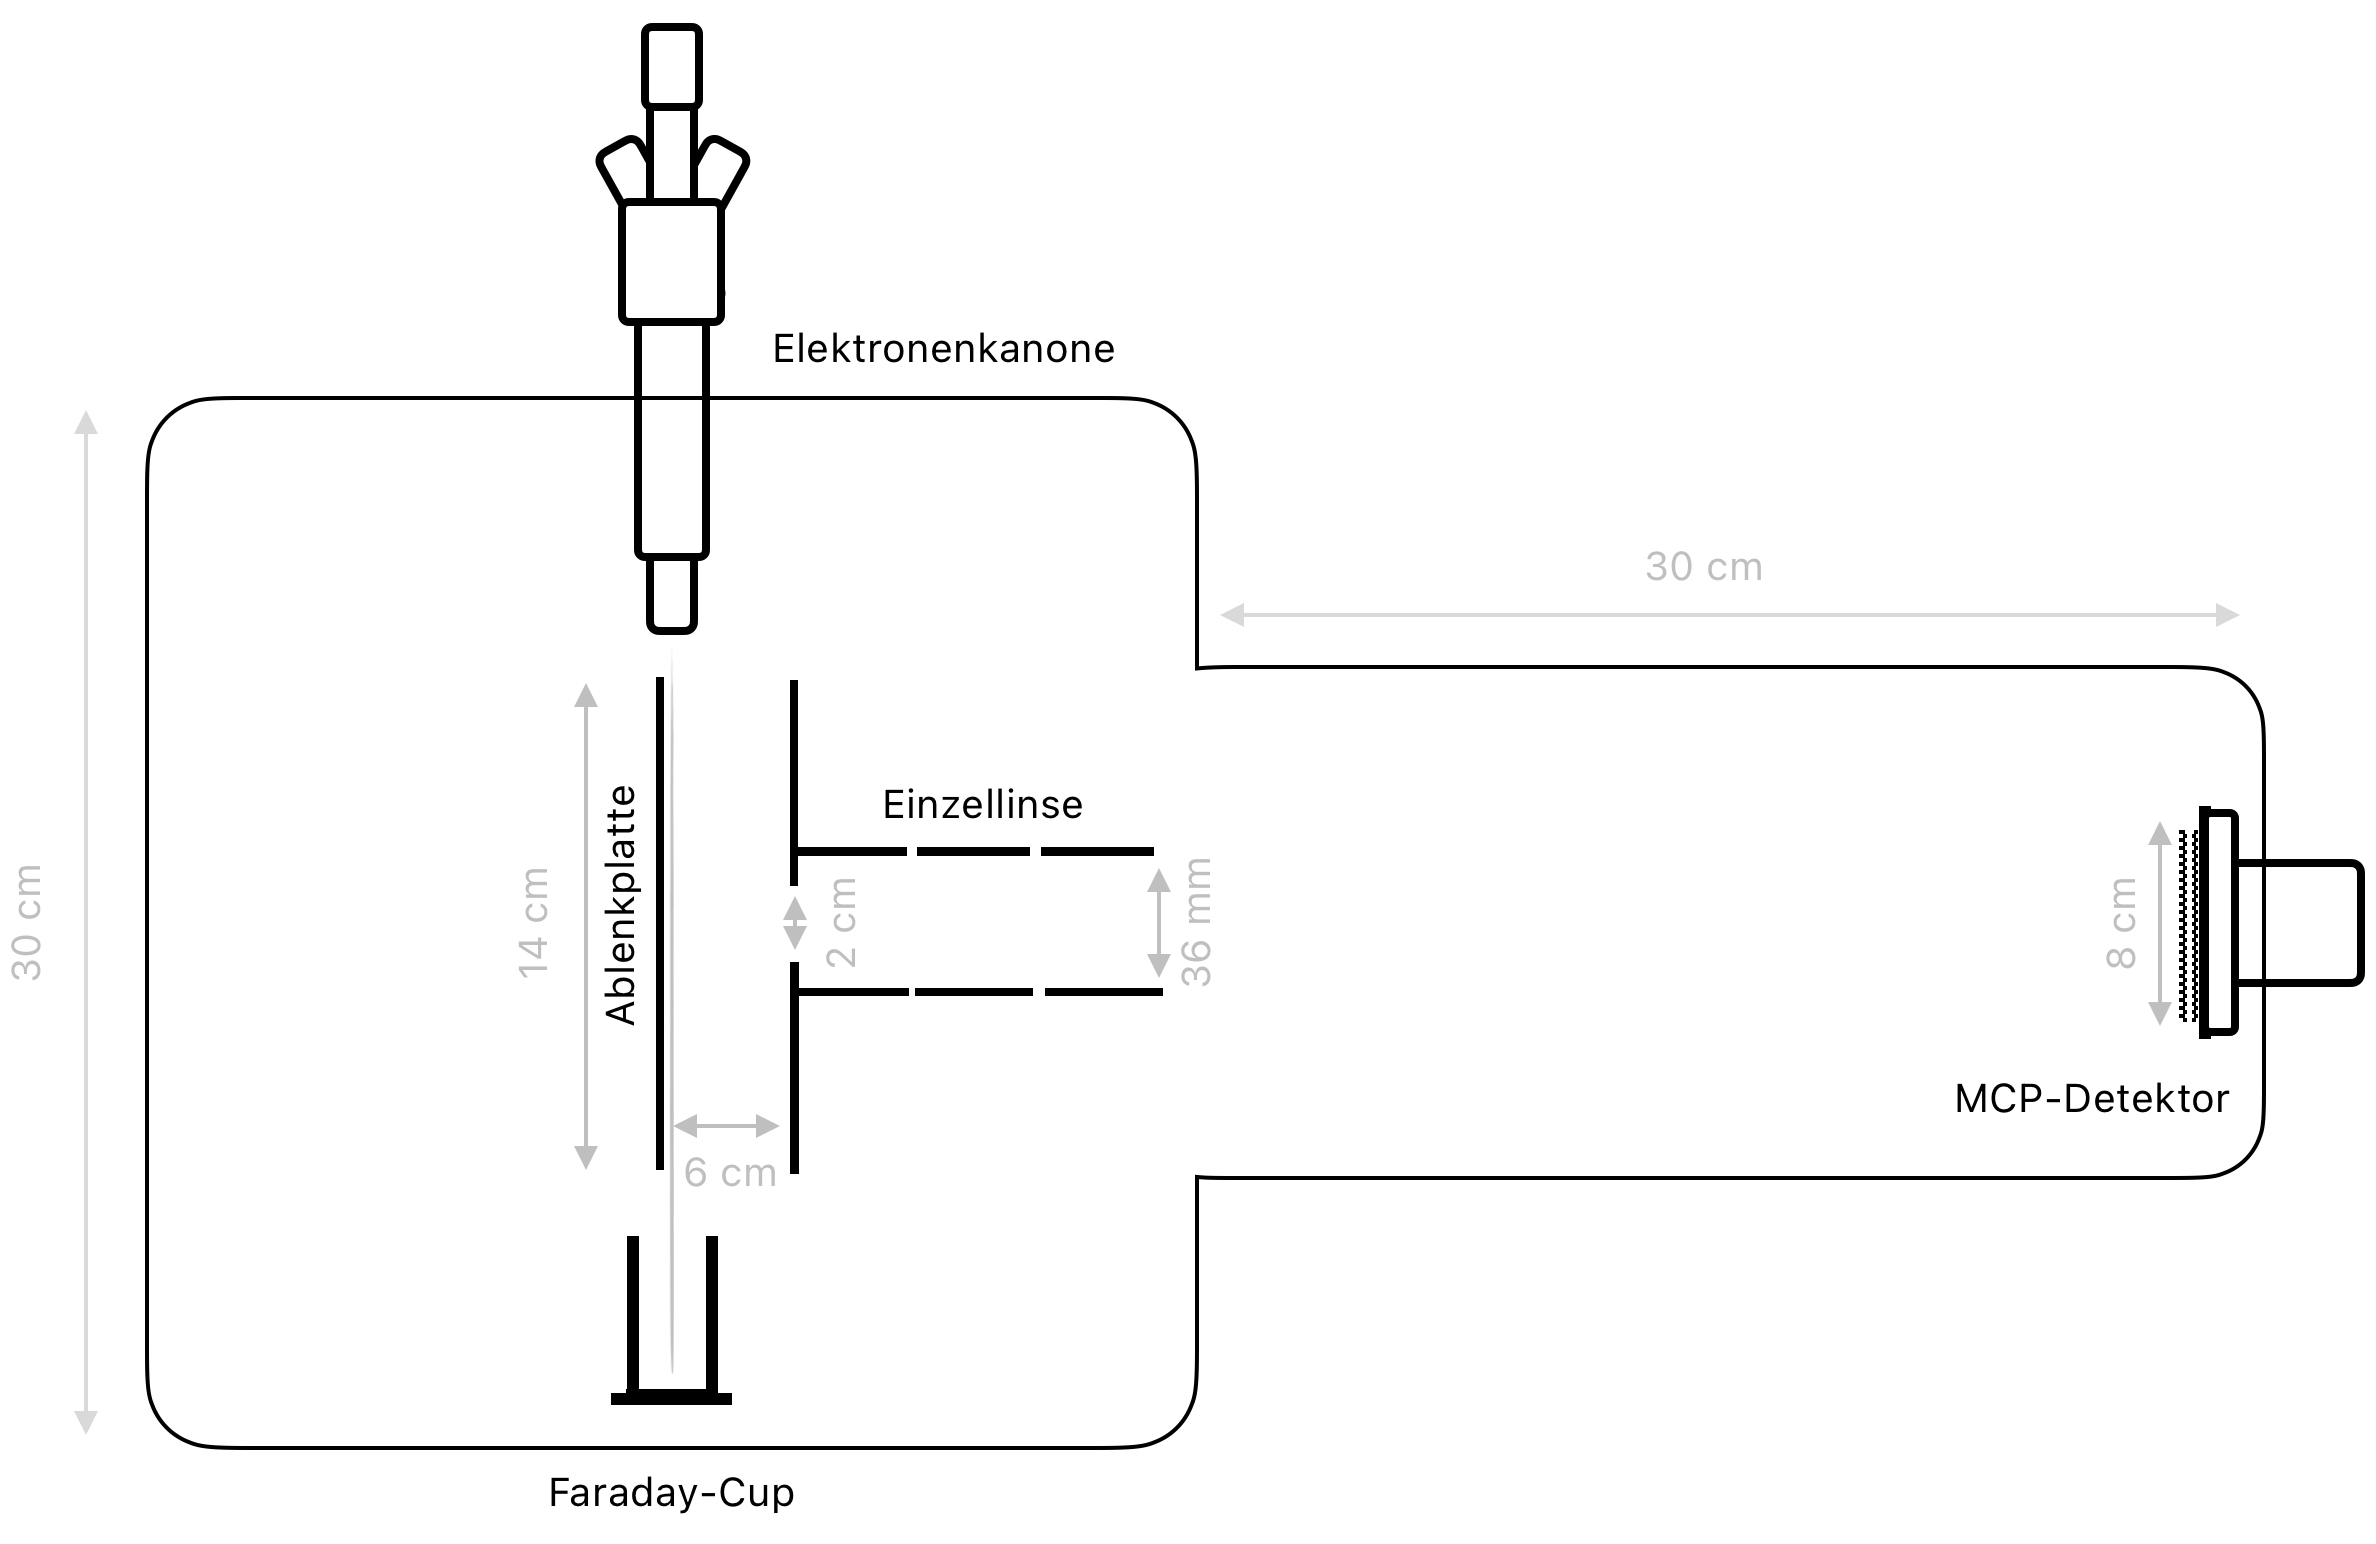
\includegraphics[width=1.5\textwidth]{SchematischerAufbau.png}
        \caption[Schematischer Aufbau des Experiments]{Schematischer Aufbau des Elektronenstoß-Experiments in der Vakuumkammer \textit{Zero-B}. Die Elektronen werden von der Elektronenkanone erzeugt. Sie stoßen mit den Neutralgasteilchen und ionisieren diese durch Stoßionisation. Die entstehenden Ionen werden über ein elektrisches Feld von einem Plattenkondensator in Richtung der Detektorplatten beschleunigt und passieren dabei eine Einzellinse.}
        \label{fig:Aufbau}
    \end{figure}
\end{landscape}

\section{Elektronenstrahl und Ablenkplatte}
\label{sec:Elektronenstrahl}
Für die Elektronenstoßionisation ist eine Heizkathoden-Elektronenkanone an einer der seitlichen Flange verbaut. Dabei handelt es sich um ein energieverstellbares Gerät von Kimball Physics, die ELG-2/EGPS-1022. Es kann einen Energiebereich zwischen 1 eV bis 2 keV abdecken. Der Strahl ist in der Ebene ablenkbar und kann variabel fokussiert werden. Die thermische Energieschärfe der verschossenen Elektronen beträgt 0.5 eV bei der Verwendung einer Tantal-Heitzkathode. Außerdem ist es möglich die Kanone in einem gepulsten Betrieb zu benutzen, was für dieses Experiment benötig wird. Dabei werden die Elektronen von einer Gitterspannung abgebremst und nur über Spannungspulse für kurze Strahldauern durchgelassen. Die Frequenz darf 5 kHz nicht überschreiten. Die Fleckgröße wird vom Hersteller als 0.5 - 5 mm im Fokuspunkt angegeben. Einen Querschnitt der Elektronenkanone zeigt Abbildung \ref{fig:EGun}. Eingestellt werden kann die Kanone über eine mitgelieferte Steuerungseinheit. Um eine optimale Fokussierung zu finden, muss für jede Energie die Anoden- und Fokusspannung angepasst werden. Während dieser Arbeit stellte sich heraus, dass Elektronenkanone eine Reperatur braucht, da die Heizkathode nicht mehr ordnungsgemäß funktioniert.

\begin{figure}
    \centering
    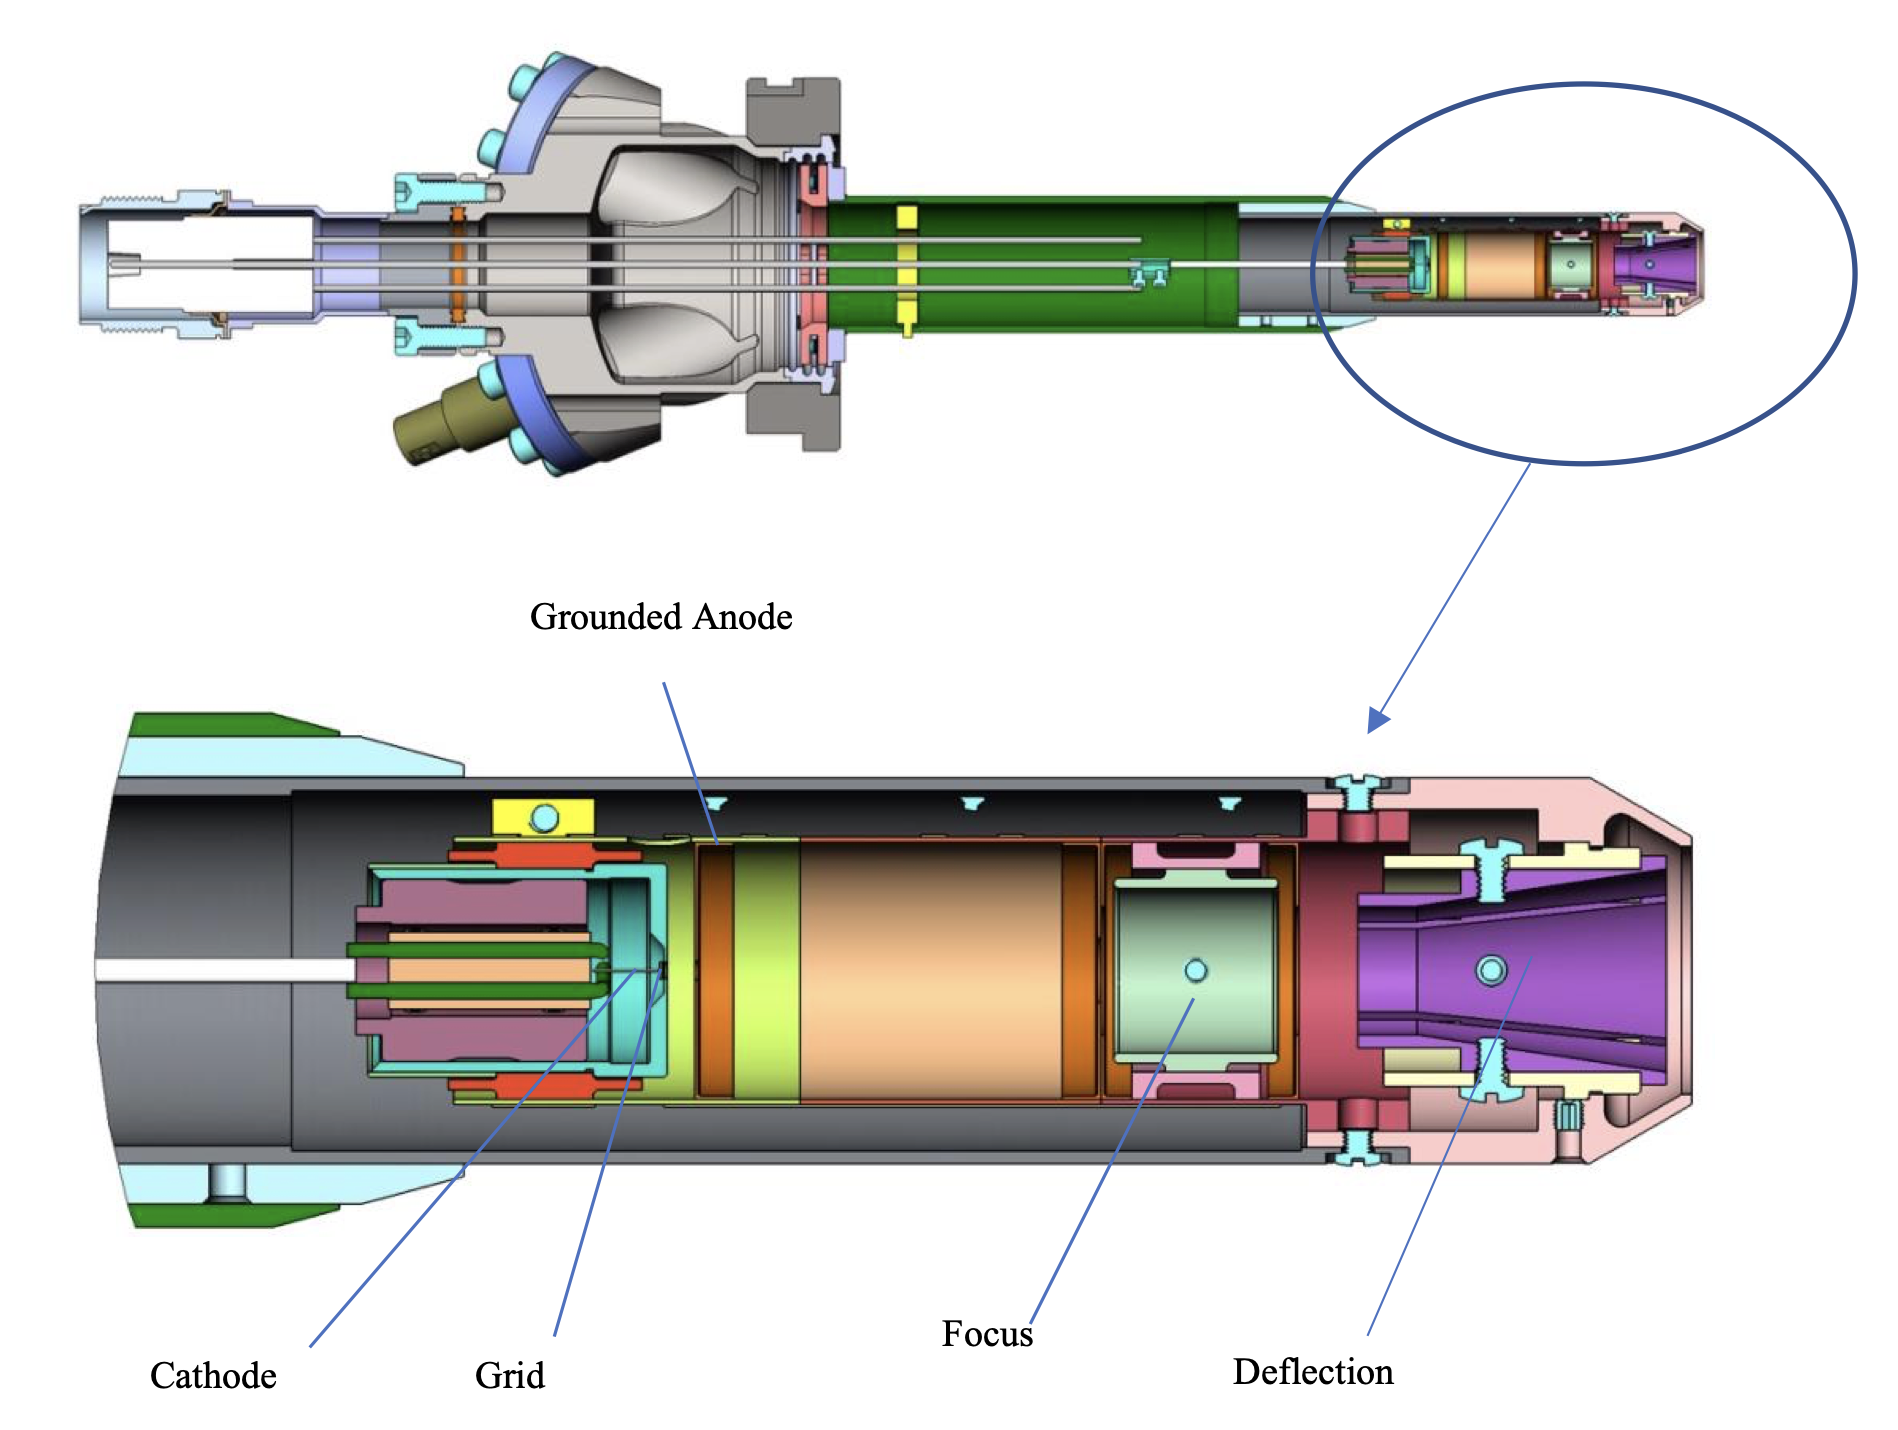
\includegraphics[width=.8\textwidth]{EGun.png}
    \caption[Querschnitt der \textsc{firing unit} der Elektronenkanone]{Querschnitt der \textsc{firing unit} der Elektronenkanone von Kimball Physics. Die Elektronen werden durch eine Heizkathode (Cathode) erzeugt und durch eine Spannung (Anode) beschleunigt. Das Gitter (Grid) kann genutzt werden, um den Extraktionsstrom der Kanone zu Pulse. Die Elektronen können fokussiert und abgelenkt werden.}
    \label{fig:EGun}
\end{figure}

Der Kanone gegenüber ist ein Faraday-Cup angebracht. Mit diesem kann die tatsächliche, momentane Elektronenstromstärke gemessen werden. Eine genaue Messung des Elektronenstroms ist für eine Messung des Wirkungsquerschnittes und für das Finden eines guten Arbeitspunktes für die Elektronenkanone essenziell. Der Faraday-Cup ist ein Metallzylinder, der von einem Isolator umgeben ist und dient als einfaches Ladungsgefäß. Er ist mit einem Elektrometer, dem DDPCA-300 von \textsc{FEMTO}, verbunden, welches den Strom und die Ladung auf dem Cup im Femto-Ampere und Pico-Coulomb Bereich messen kann. Für die Messung der Ladung ist es wichtig, dass die von der Elektronenkanone im gepulsten Betrieb akkumulierte Ladung dem Rauschen deutlich überwiegt. Deshalb ist es, besonders für geringe Elektronenenergien, lohnenswert den Elektronenstrom bestmöglich einzustellen und ein rauscharmes Kabel zu verwenden. Für diese Messung wurde ein besonders großer Faraday-Cup mit einem Durchmesser von 30 mm und einer Tiefe von ca. 80 mm verwendet. Das hat zwei Gründe: Zum einen ist die Fläche des Cups groß genug, um den gesamten Elektronenstrom aufzufangen - auch wenn er nicht perfekt fokussiert ist oder vom magnetischen Restfeld abgelenkt wurde, was essenziell für die Messung ist. Zum anderen ist die Tiefe des Cups möglichst groß gewählt, damit es unwahrscheinlicher ist, dass aus dem Cup durch Stoßionisation entstandene Ionen und Sekundärelektronen in die Kammer gelangen. Von dem sonst aus diesem Grund verwendeten Repeller-Ring wurde abgesehen, da das elektrische Feld Einfluss auf die Messung nehmen könnte.

In der Mitte der Kammer durchquert der Strahl einen zylindrischen Plattenkondesator, wobei er die Bodenplatte mit einem Abstand von etwa 1.5 cm parallel passiert. Auf der Bodenplatte kann über einen Hochspannungspulsgenerator (PVX-4130) ein elektrisches Feld angelegt, um die Ionisationsprodukte auf die Detektorplatten zu beschleunigen. Dieser kann hochfrequente Pulse von bis zu 6 kV mit einer Flankenanstiegszeit von wenigen Nanosekunden erzeugen. Der Spannungspuls wird leicht verzögert ausgelöst. Die Deckenplatte hat in der Mitte ein kreisförmiges Loch mit 2 cm Durchmesser, durch das die Ionen Richtung Detektor gelangen. Auf diesem befindet sich ein Goldnetz (88 \% Transparenz), das Restfelder hinter dem Plattenkondensator reduzieren soll. Die Frontplatte des Detektors liegt, wie im nächsten Abschnitt genauer beschrieben, auf einem negativen Potential von -2.5 kV, sodass sich bei einem Spannungspuls von 4 kV und einem einfach geladenen Ion in etwa eine kinetische Energie $E_{kin} = e \cdot (U_{Detektor} - U_{Kondensator}) = 6.5$ keV ergibt. Ein 3D-Modell der Kammer mit dem Plattenkondensator ist in Abbildung \ref{fig:3D} zu sehen.

\begin{figure}
    \centering
    \hspace{-2.8cm}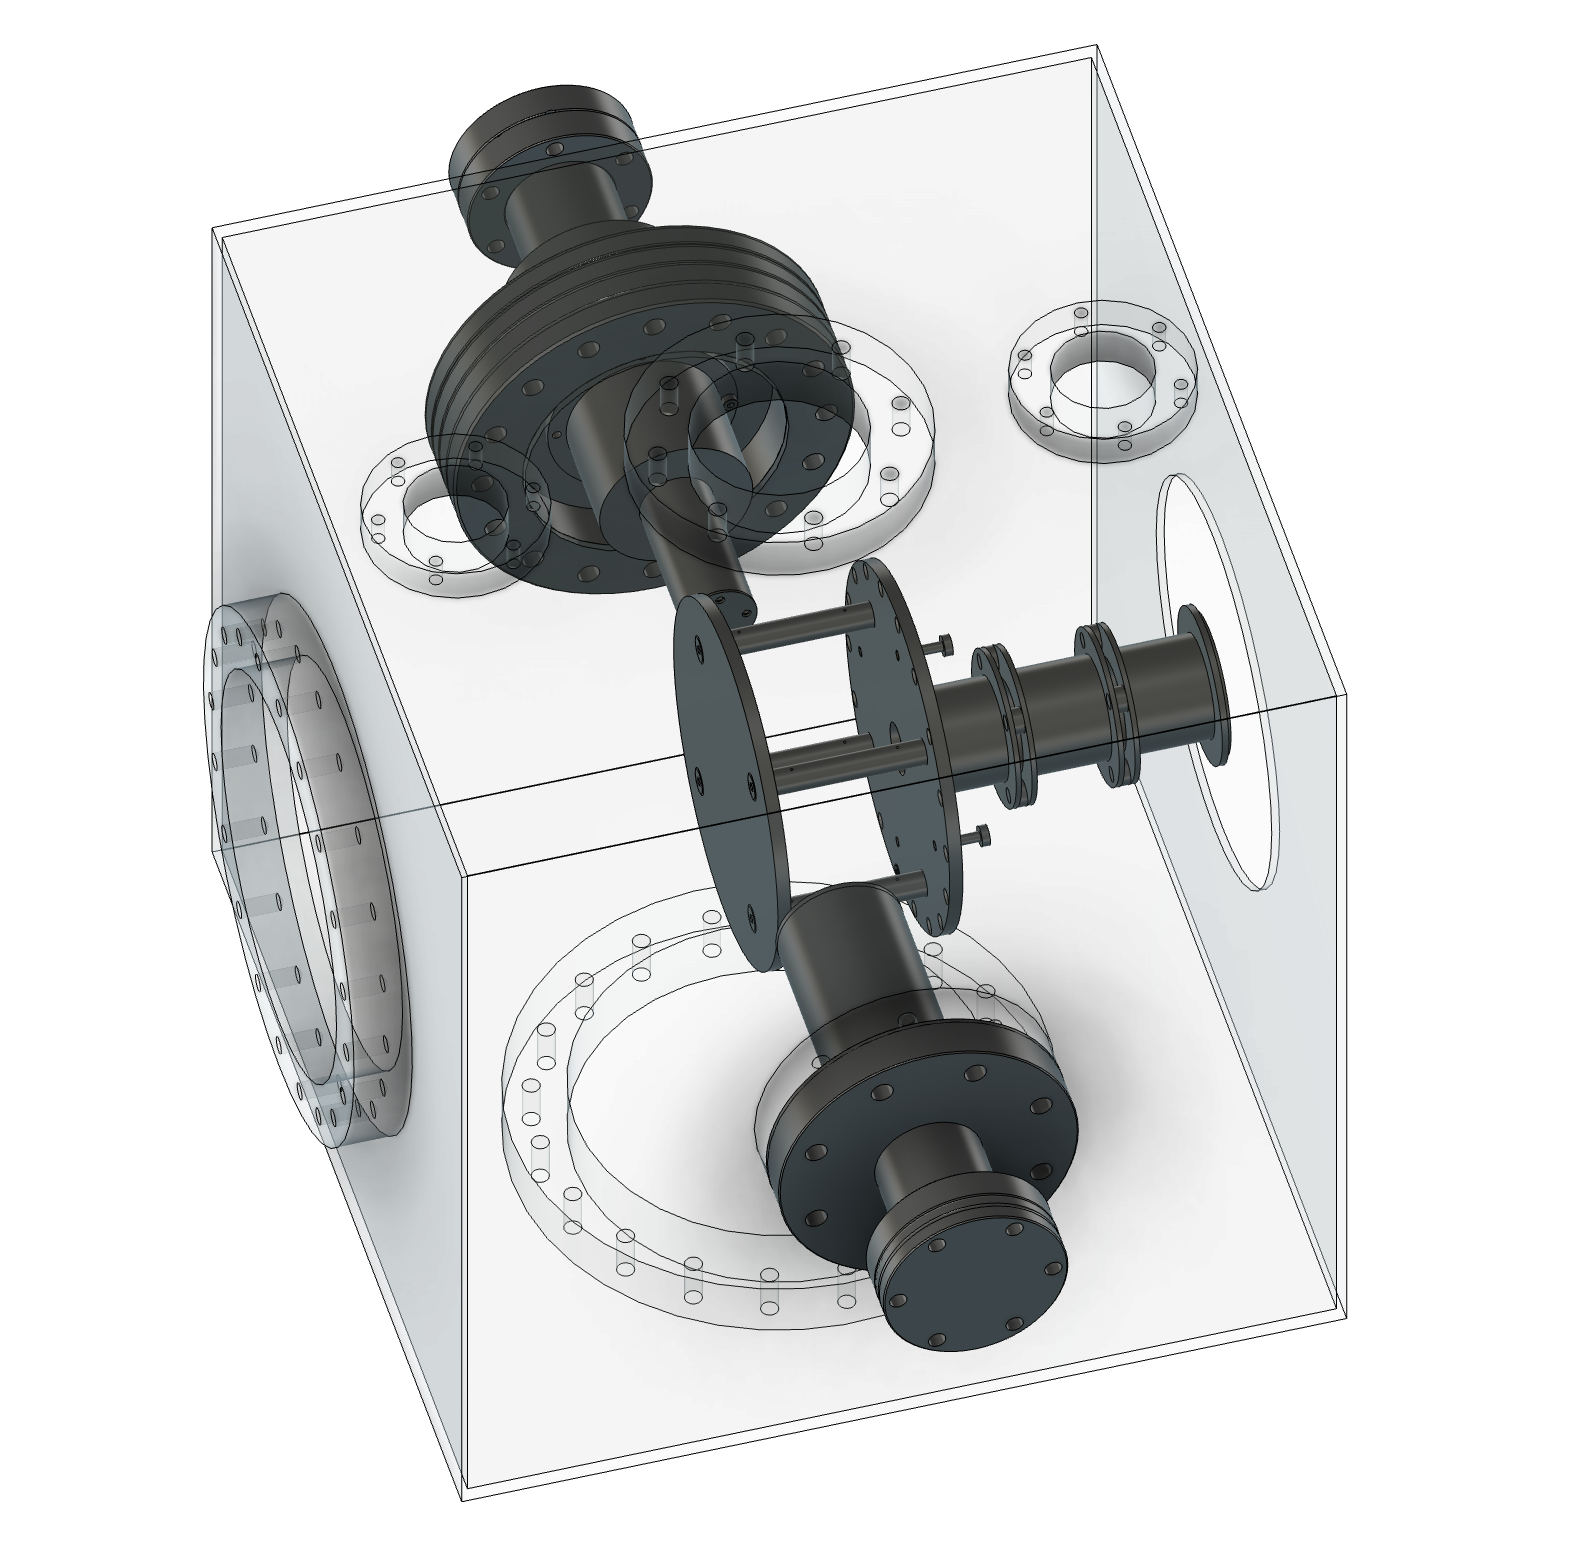
\includegraphics[width=1.2\textwidth]{Kammer_3D.png}
    \caption[3D-Modell der Vakuumkammer mit Plattenkondensator]{3D-Modell der Vakuumkammer mit Plattenkondensator. Auf der dem Betrachter zugewandten Seite ist der Faraday-Cup zu sehen, gegenüber die Elektronenkanone. Der Strahl durchquert den zylindrischen Plattenkondensator (Bodenplatte links) in der Mitte und die Produkte werden durch eine elektrische Einzellinse (drei Zylinder, rechts) hindurch auf die Detektorplatten (nicht abgebildet) extrahiert. Durchsichtig abgebildet sind die Seitenwände der Kammer.}
    \label{fig:3D}
\end{figure}

\section{Detektorsystem}
Bei dem in dieser Arbeit verwendeten Detektor handelt es sich um einen positionssensitiven Mikrokanalplattendetektor (MCP-Detektor) der Firma Roentdek. MCP-Detektoren sind eine verbreitete Detektortechnologie, die es ermöglicht den Auftreffzeitpunkt von einzelnen Ionen, Elektronen oder Photonen zu bestimmen. Mit einer Widerstandsanode kann die Position der durch die Platten verstärkten Signale anschließend bestimmt werden. So kann ein Bild der detektierten Teilchen erzeugt werden. Im Versuchsaufbau schirmt das in Kapitel \ref{sec:Elektronenstrahl} erwähnte Goldnetz den Detektor von elektromagnetischen Störungen und Restfeldern ab. Die für den Detektor typischen Leistungsparameter sind in Tabelle \ref{tab:MCP} aufgeführt. Der für das Experiment verwendete Detektor ist ein delay-line Detektor, genauer der DLD80.


% table of typical values for MCP detectors
\begin{table}[h]
    \centering
    \caption{Von Roentdek angegebene typische Parameter für den MCP-Detektor}
    \begin{tabular}{c|c}
        Parameter & Wert \\
        \hline
        Aktive Fläche & 80 mm \\
        Effizienz & $>$ 50 \% \\
        räumliche Auflösung & $<$ 0.1 mm \\
        Zeitauflösung & $<$ 0.2 ns \\
        maximale Rate & 1 MHz \\
        Totzeit & 10-20 ns \\
        Kanaldurchmesser & 25 $\mu$m \\
        Plattendicke & 1.5 mm \\
        Vorzugswinkel & \ang{8} $\pm$ \ang{1} \\

    \end{tabular}
    \label{tab:MCP}
\end{table}

\subsection{Mikrokanalplatten}
Die Mikrokanalplatten des Detektors dienen der Verstärkung von eintreffenden Signalen über die Erzeugung von Sekundärelektronen. Sie bestehen aus Glas, welches mit einer sehr hohen Dichte von kleinen, geraden Kanälen durchzogen ist, welche die gegenüberliegenden Seiten verbinden. Bei der Herstellung wird das Glas dafür, ähnlich wie bei der Herstellung von Glasfasern, gezogen und in Millimeterdicke Scheiben geschnitten. Der Durchmesser der Kanäle liegt bei einigen Mikrometern. Die Innenwände der Kanäle bestehen aus einem halbleitenden Material, an welches eine Spannung entlang der Kanäle angelegt wird. Diese beschleunigt die Elektronen entlang des Kanals. Trifft ein Teilchen auf die Wand eines Kanals der Detektorplatten, löst es durch Stoßionisation Sekundärelektronen aus. Diese werden durch das elektrische Feld beschleunigt und ionisieren weitere Atome oder Moleküle beim Aufprall auf die Kanalwand. Dieser Prozess setzt sich fort und führt zu einer Elektronenlawine, die als Townsend-Lawine bekannt ist. Das Prinzip ist in Abbildung \ref{fig:MCP} dargestellt. Dieser verstärkende Effekt wird sich zunutze gemacht, um aus einzelnen Teilchen eine messbare Ladungswolke zu erzeugen. Um die Wahrscheinlichkeit einer Kollision einfallender Teilchen mit den Kanalwänden zu steigern, sind die Kanäle um etwa \ang{8} gegenüber der Flächennormalen geneigt. 

\begin{figure}
    \centering
    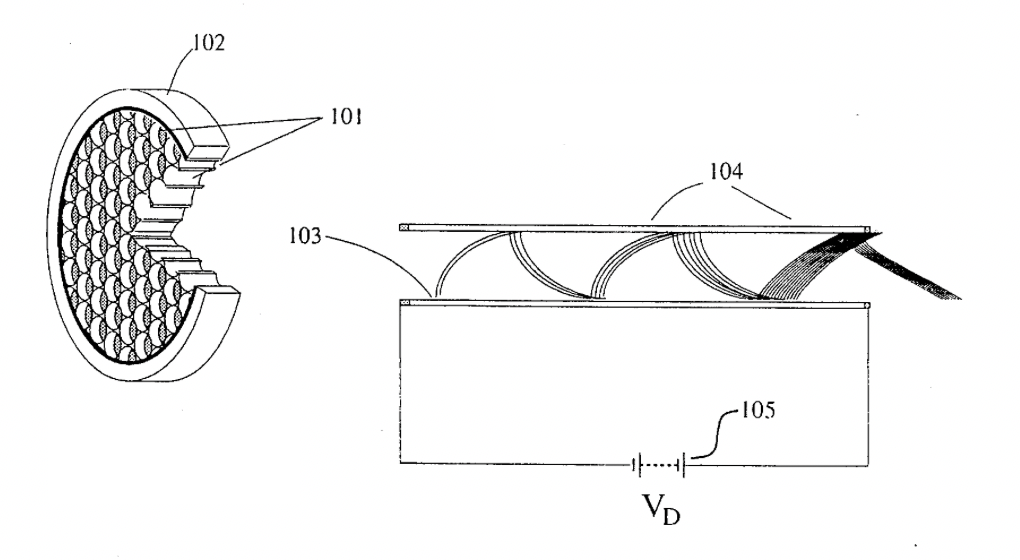
\includegraphics[width=.7\textwidth]{MCP.png}
    \caption[Schnitt und Funktionsprinzip einer MCP]{Schnitt und Funktionsprinzip einer MCP aus \cite{MCP}, hier dargestellt mit einem eintretenden Elektron. (102) Haltungsflange, (101) Mikrokanäle aus Glas, (103) Elektron, welches in den Kanal eintritt, (104) erzeugte Sekundärelektronen, (105) Spannungsversorgung der Platten}
    \label{fig:MCP} 
\end{figure}

Typischerweise werden zwei MCPs hintereinander verwendet, wobei sie um \ang{180} zueinander gedreht sind. Sie befinden sich in einer sogenannten \textsc{Chevron}-Konfiguration. Die zweite Platte wird verwendet, um die Verstärkung weiter zu erhöhen und Ionen-Feedback zu minimieren. Ionen-Feedback beschreibt das Zurückfließen von Ionen in die Kammer. Die hohe Anzahl an Elektronen in den Kanälen der MCPs können Restgas ionisieren, welches dann, aufgrund der Beschleunigungsspannung, rückwärts durch die Kanäle in die Kammer gelangen könnte. 

\begin{figure}
    \centering
    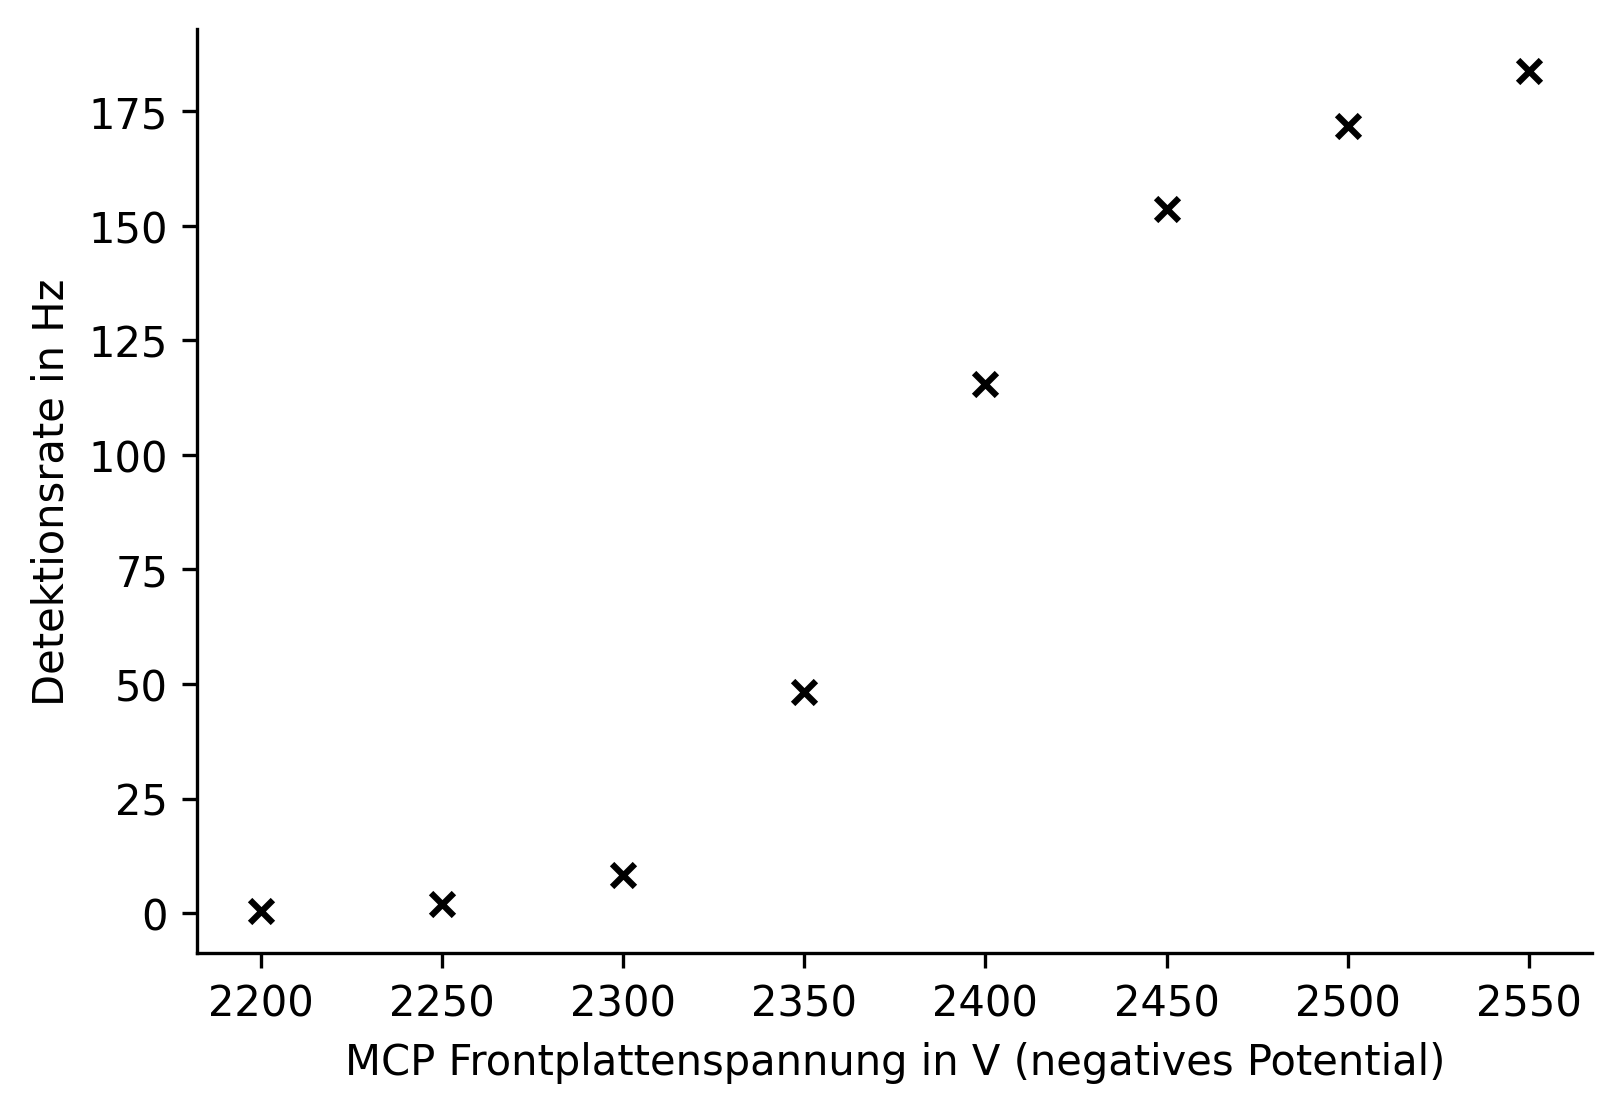
\includegraphics[width=.6\textwidth]{MCP_Sensitivity.png}
    \caption[Detektionsrate in Abhängigkeit der Frontplattenspannung]{Detektionsrate in Abhängigkeit der Frontplattenspannung. Die Rate steigt ab einem negativem Potential von 2300 V stark an und erreicht erst bei einer Spannung größer 2550 V ein Plateau}
    \label{fig:Frontplattenspannung}
\end{figure}

Die auf die Frontplatte angelegte Spannung bestimmt, mit welcher Energie die Ionen auf die Platte treffen. Im Optimalfall sollte sie so hoch einstellt werden, dass die Detektionsrate unabhängig von der Spannung wird. Ziel ist, das alle auf den Dektektor treffenden Ionen genügend Energie haben, um Elektronen auszulösen und somit detektiert zu werden. Abbildung \ref{fig:Frontplattenspannung} zeigt den Zusammenhang von Frontplattenspannung und Detektionsrate. Sie bildet das Ergebnis einer Messreihe der Counts bei konstantem Gasdruck und Elektronenstrahlparametern bei verschiedenen MCP-Spannungen ab. Um die Rate zu erhalten werden die Counts durch die Zeit der Messung geteilt. Anhand der Werte ist zu erkennen, dass es nicht möglich ist, mit diesem MCP-Detektor vollständig in der Sättigung zu arbeiten, wenn der empfohlene Spannungsbereich eingehalten wird, da auch bei maximaler Spannung eine Erhöhung der Spannung zu einer Erhöhung in der Rate führt. Trotzdem nimmt diese Zunahme bei einer Spannung größer als 2400 V ab. Bei der Aufnahme sämtlicher Daten werden im Folgenden deshalb Spannungen größer 2400 V gewählt, um möglichst viele Ionen nachweisen zu können.

\subsection{Positionsbestimmung}
Wie in \cite{Detektorsystem} dargestellt, gibt es unterschiedliche Ansätze die zweidimensionale Positionsinformation der durch die Platten erzeugten Ladungswolke zu ermitteln. Das hier verwendete Konzept macht sich zu Nutzen, dass eine auf ein Drahtgitter treffende Ladungswolke ein elektrisches Signal in den Leitern erzeugt. Dieses hat eine Laufzeit in der Größenordnung einiger Nanosekunde bis es an den Enden des Leiters ankommt. Anhand dieser Laufzeitdifferenz kann die Position auf dem Detektor in einer Dimension bestimmt werden. Mithilfe eines zweiten, um \ang{90} gedrehten, Leiters, kann die Position zweidimensional dargestellt werden. In Abbildung \ref{fig:DLD} ist die Drahtstruktur für die Messung einer Dimension gezeigt. Der Detektor hat eine aktive Fläche mit einem Durchmesser von 80 mm. In dieser Arbeit ist die Bestimmung der Auftreffpositionen zweitrangig und wird in erster Linie dafür verwendet zu validieren, dass die Ionen tatsächlich primär aus der Elektronenstoßionisation stammen und nicht zufällig verteilt sind. Der Ursprung der Ionen wird auf dem Bild des Detektors indirekt abgebildet und zeigt deutlich den Strahl der Elektronenkanone. Die Auswertung der Positionsbestimmung erfolgt in Kapitel \ref{chap:Auswertung} zur Auswertung.

\begin{figure}
    \centering
    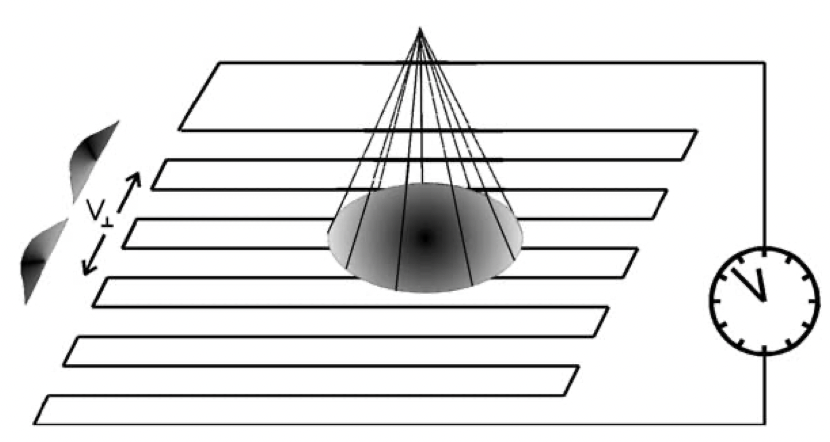
\includegraphics[width=.5\textwidth]{DLD.png}
    \caption[Funktionsprinzip der Laufzeitmessung des Detektors]{Funktionsprinzip der Laufzeitmessung in einer Dimension aus \cite{Detektorsystem}. Der Leiter ist mäanderförmig aufgebaut, um die Laufzeit zu verlängern und die Positionsgenauigkeit zu erhöhen. Das Signal propagiert in beide Richtungen mit der effektiven Geschwindigkeit $v_\perp$.}
    \label{fig:DLD} 
\end{figure}

\section{Konditionierung des Detektors}
Nachdem der Detektor eingebaut ist, muss er einer Konditionierung unterzogen werden, damit er verwendet werden kann, ohne das Risiko beschädigt zu werden. Zur Konditionierung soll die Spannung zwischen den MCPs in 100 V Schritten erhöht werden und je für einige Minuten konstant gelassen werden. Das hat den Hintergrund, dass Partikel, wie zum Beispiel Staubteilchen, sich von den MCPs oder Teilen des Detektors lösen können und bei schnellem Ansteigen der Spannung Schäden an den Platten hinterlassen können. Beim Konditionieren können diese Partikel sich nach und nach lösen und bekommen nur minimale kinetische Energie zugeführt. Außerdem können Überschläge bei möglichst geringer Potenzialdifferenz festgestellt werden, welche ebenfalls von Partikeln begünstigt werden können. Für die Spannungsversorgung der Detektorplatten wird eine Hochspannungsquelle verwendet, die mit einem Überstromschutz bei sprunghaft ansteigendem Strom abschaltet. Die Konditionierung wird im Vakuum über mehrere Stunden bis zu einer Potenzialdifferenz von 2.7 kV durchgeführt. Nach jedem Erhöhen der Spannung wird der sich eingestellte Strom notiert und der Widerstand berechnet, welcher in etwa konstant bleiben oder sich mit steigender Spannung etwas verkleinern sollte. Tabelle \ref{tab:Konditionierung} im Anhang zeigt die notierten Werte für die Konditionierung ab 880 V, welche ohne Probleme durchgeführt werden konnte. Nach einmaliger Konditionierung kann der Detektor mit einer Geschwindigkeit von etwa 40 V/s ohne weiteres hochgefahren werden.

\section{Signalverarbeitung}
Die auf der Anode des Detektors entstehenden Signale müssen weiterverarbeitet werden, um sie für die Auswertung zu nutzen. Ein Großteil der Signalverarbeitung wird in dieser Arbeit analog umgesetzt. Viele der verwendeten Geräte sind ältere, aber verlässliche Nuclear Instrumentation Module (NIM). Diese können sehr modular in einem Rack verbaut und über BNC-Kabel verbunden werden. Im Folgenden wird die Signalverarbeitung zur Flugzeitmessung und die zur positionssensitiven Auflösung der Ionen unterschieden.

\subsection{Flugzeitmessung}
Eine schematische Übersicht der Verarbeitung ist in Abbildung \ref{fig:ToF} zu finden. Der Signalfluß, angefangen mit dem Startsignal wird nun beschrieben.
\begin{figure} 
    \centering
    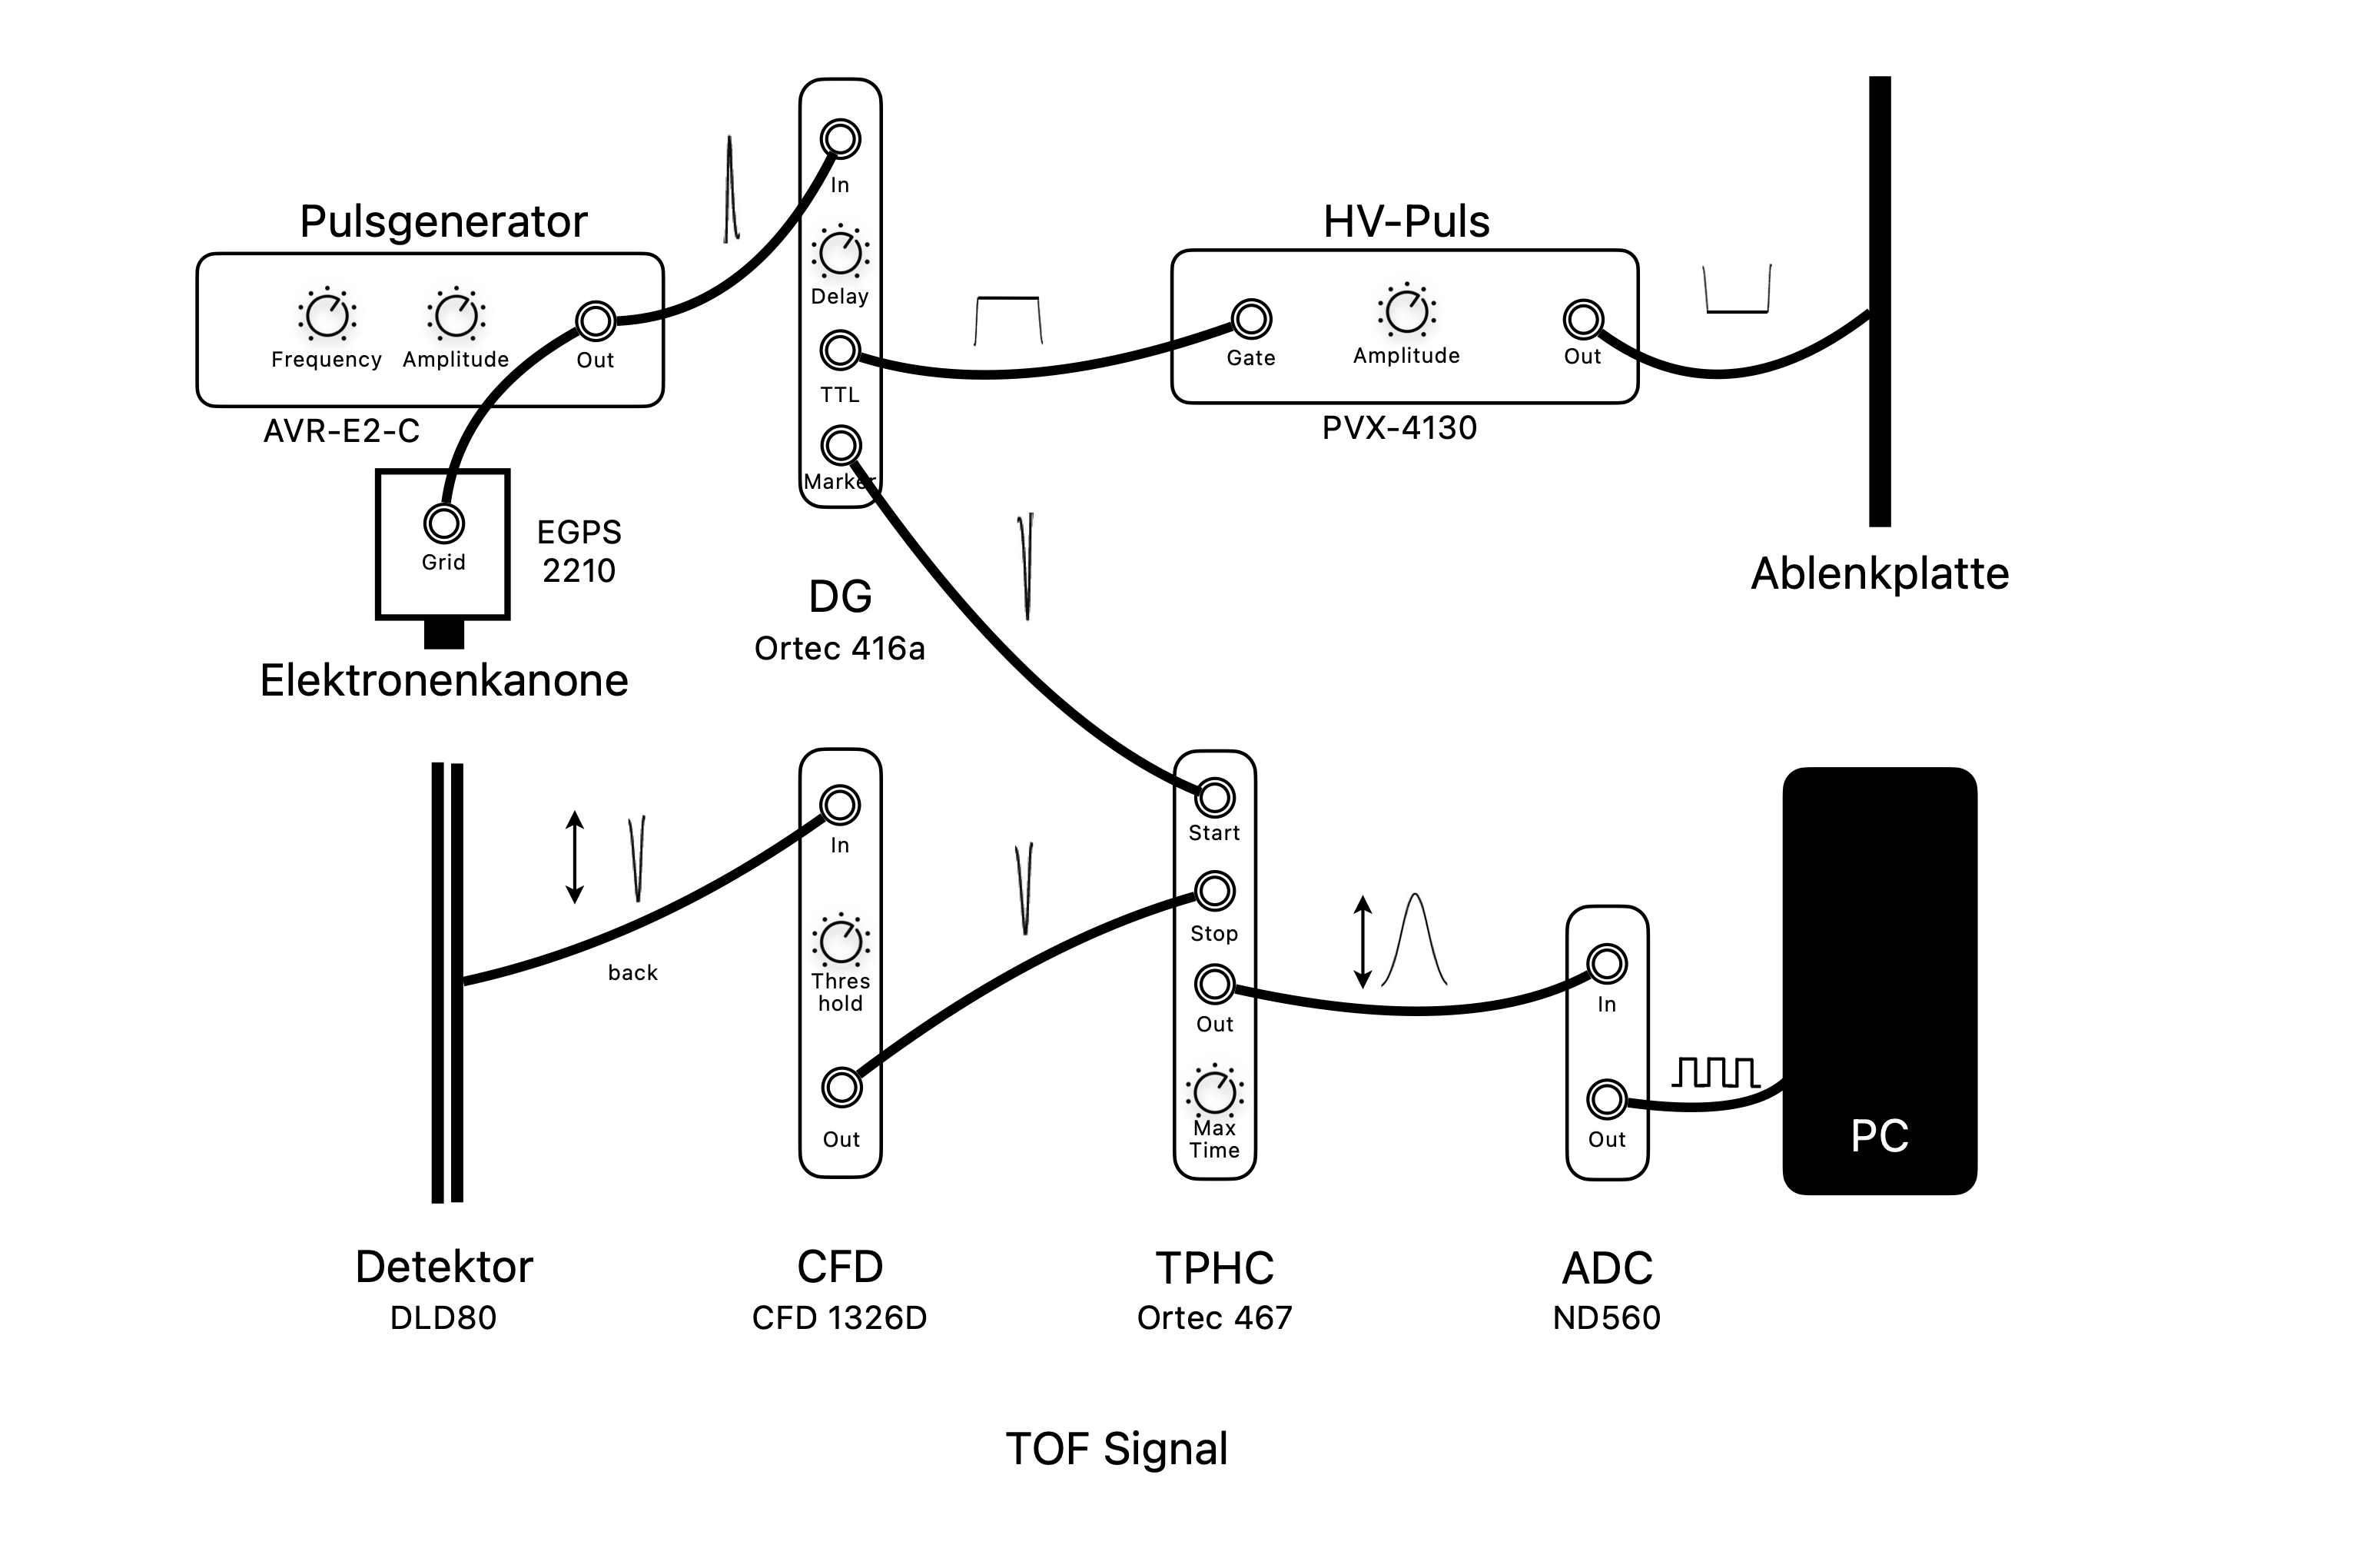
\includegraphics[width=.95\textwidth]{ToF_Signals.png}
    \caption[Schematisch dargestellter Signalfluß der ToF-Messung]{Schematisch dargestellter Signalfluß der ToF-Messung. Der Signalfluß erfolgt, mit Ausname der Elektronenkanone, von links nach rechts. Die verwendeten Geräte sind stark vereinfacht abgebildet, wobei die wichtigsten Einstellungen inkludiert wurden. Die jeweilige Form der Signale ist über den Verbindungen gezeigt und ist rein qualitativ. Power Supplies sowie Anzeigegeräte sind nicht abgebildet.}
    \label{fig:ToF} 
\end{figure}
Um das Startsignal zu erzeugen und die Flugzeitmessung überhaupt in Gang zu setzen, wird ein Pulsgenerator verwendet. Dabei handelt es sich um den AVR-E2-C von AVTECH. Die erzeugten Pulse werden direkt zum triggern der Elektronenkanone verwendet und über einen Delay-Generator (DG) verzögert. Der DG kann sehr genau auf eine Verzögerung einiger Nanosekunden eingestellt werden. Damit ein DG Verzögerungen realisieren kann, wird eine stabile Frequenz benötigt. Diese wird meist durch einen Quarzoszillator erzeugt, ein Kristall über den AC-Pulse angelegt werden. Dieser vibriert mit seiner Resonanzfreuqenz aufgrund des Piezo-Effekts und ermöglicht eine genaue Messung der Zeit. Der TTL-Output des DG wird dann verwendet, um die Ablenkspannung für die Ionen zu erzeugen. Gleichzeitig wird ein Marker (scharfer Puls) ausgegeben, der als Startsignal für die Flugzeitmessung verwendet wird.

Für die Bestimmumg des Auftreffzeitpunktes wird vom Detektor ein Spannungssignal ausgegeben, das von einem Ion beim Auftreffen auf die Anode erzeugt wird.  Der Pegel hängt von der kinetischen Energie des Ions ab und hat eine gewisse Varianz. Der Zeitpunkt soll möglichst unabhängig vom Pegel bestimmt werden können. Wird also lediglich einen Schwellwert festgelegt, variert der Zeitpunkt mit der Steilheit der Flanke. Um den Zeitpunkt unabhängig vom Pegel zu bestimmen, wird ein Constant Fraction Discriminator (CFD) verwendet. Dieser erzeugt ein Ausgangssignal, sobald ein bestimmter Bruchteil des Signals erreicht wird. Abbildung \ref{fig:CFD} zeigt das Prinzip des CFD. Dafür wird im CFD das einlaufende Signal verzögert und mit dem Originalsignal über einen Differenzverstärker verrechnet. So ergibt sich ein Nulldurchlauf der Spannung, der von der Verzögerung abhängt, nicht aber von der Amplitude. 

\begin{figure}
    \centering
    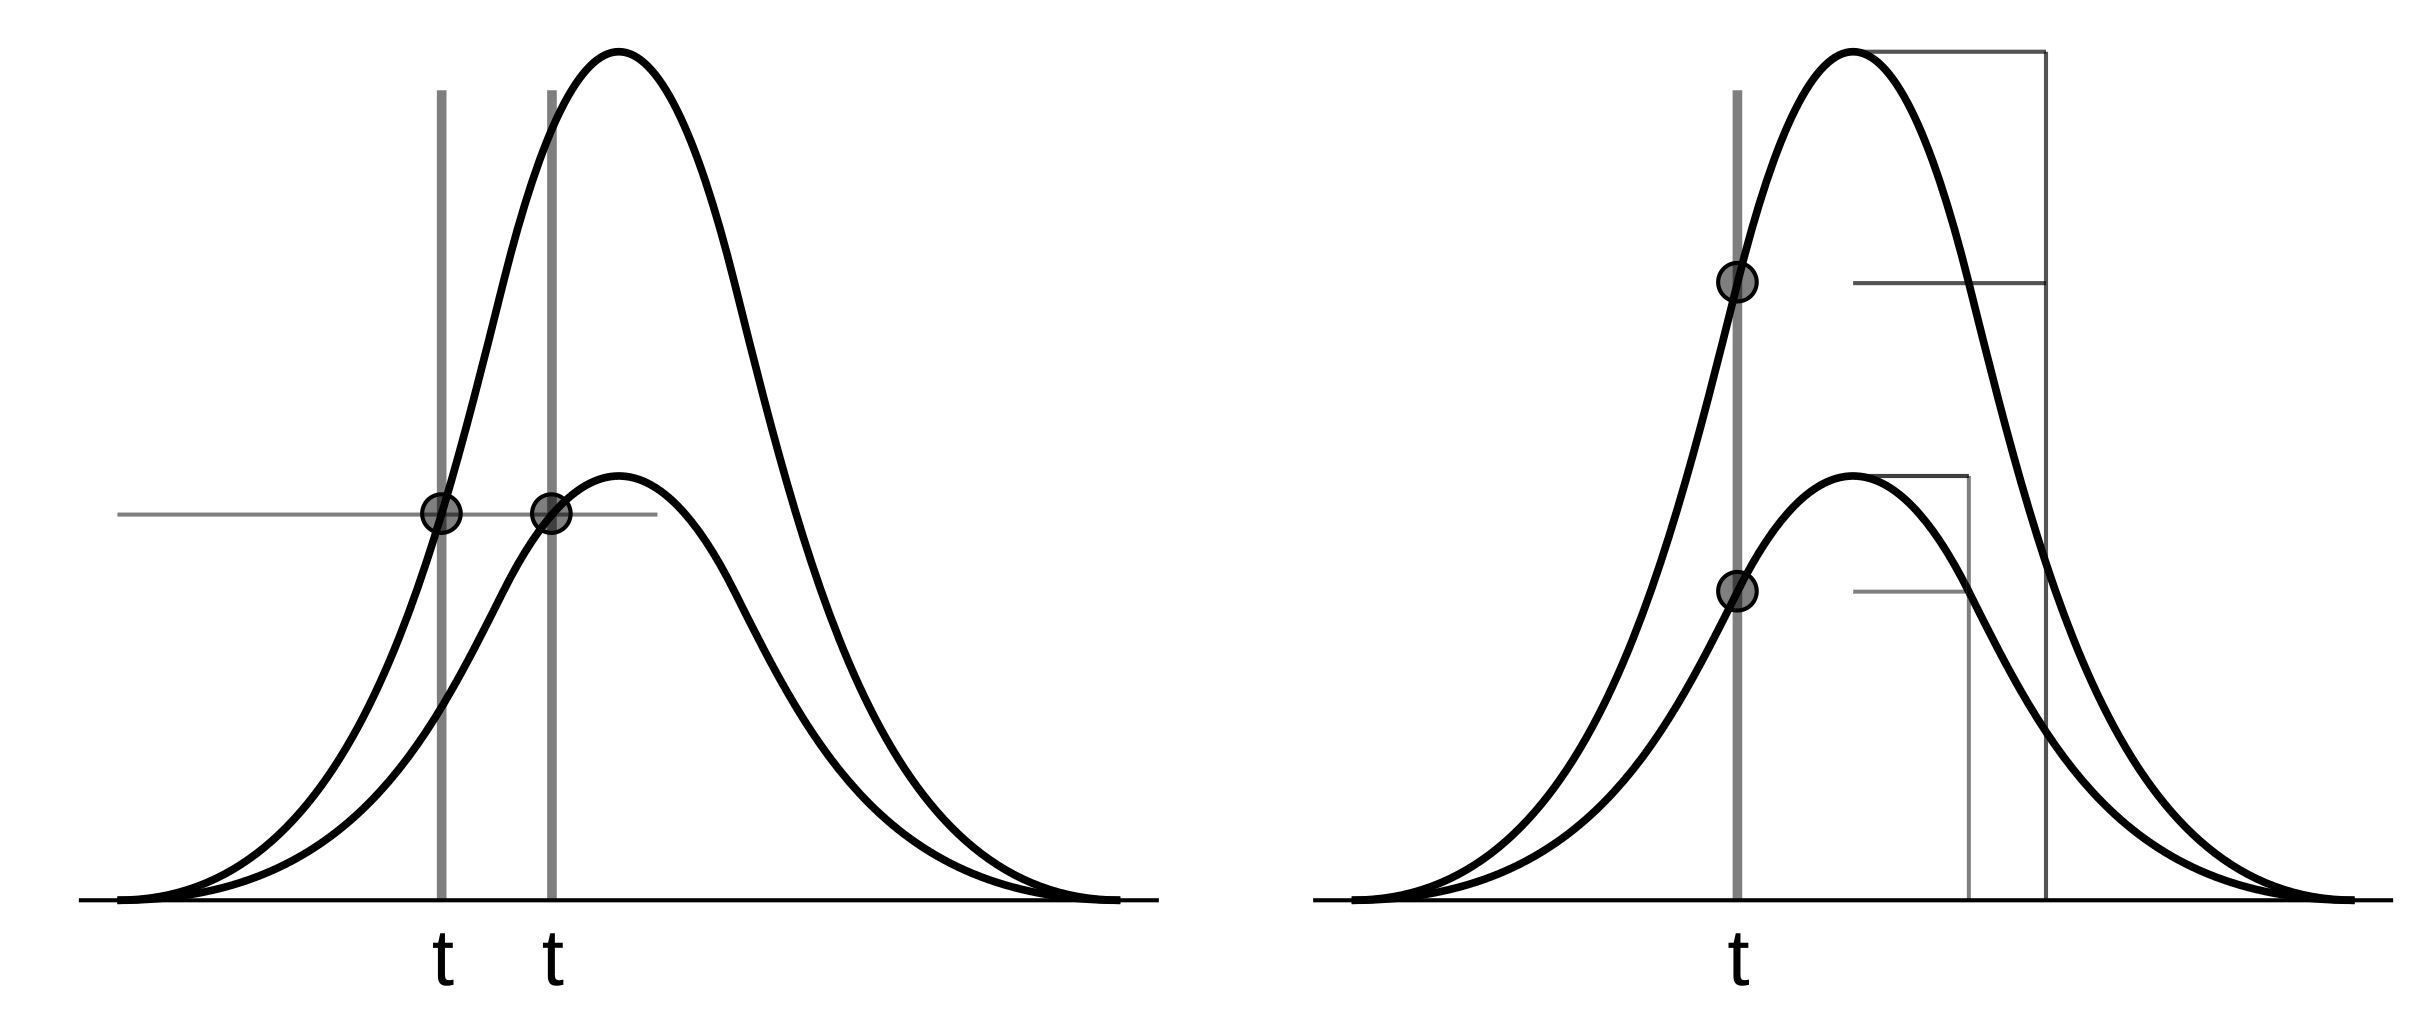
\includegraphics[width=.5\textwidth]{cfd.png}
    \caption[Prinzip des Constant Fraction Discriminators]{Prinzip des Constant Fraction Discriminators \cite{CFD}. Links: Zeitpunkte beim Überschreiten eines Schwellwertes sind unterschiedlich, rechts: Der Zeitpunkt beim Überschreiten eines Bruchteils des Signals ist unabhängig vom Pegel.\\}
    \label{fig:CFD} 
\end{figure}

Der über den CFD ermittelte Auftreffzeitpunkt kann dann als Stoppsignal für die Flugzeitmessung dienen. Um die Information über die Zeitdifferenz zwischen dem Start- und Stoppsignal zu erhalten, wird ein Time-to-Pulse-Height-Converter (TPHC) Modul verwendet. Dieses erzeugt ein Signal, dessen Höhe proportional zur zeitlichen Differenz eines Start- und Stoppulses ist. Um diese Funktionalität umzusetzen wird im TPHC ein Kondensator aufgeladen, wobei die Spannung über den Kondensator proportional zur Ladezeit steigt. Kommt kein Stoppsignal, wird der Kondensator nach einer eingestellten maximal Dauer über einen Widerstand wieder entladen. Schließlich kann der Spannungspuls über einen Analog-Digital-Converter (ADC) digitalisiert und am Computer ausgelesen werden. Abbildung \ref{fig:Signal} zeigt qualitativ den zeitlichen Verlauf der relevanten Signale der Flugzeitmessung. Anhand vieler Messungen kann ein Spektrum der Flugzeiten erstellt werden.

Dank des Pulsgenerators kann die Messung mehrere tausendmal in jeder Sekunde durchgeführt werden. Begrenzend ist dabei die Elektronenkanone, die, wie bereits erwähnt, mit maximal 5 kHz gepulst werden kann. Für die meisten Messungen wurde eine Frequenz von etwa 3 kHz verwendet.

\begin{figure}
    \centering
    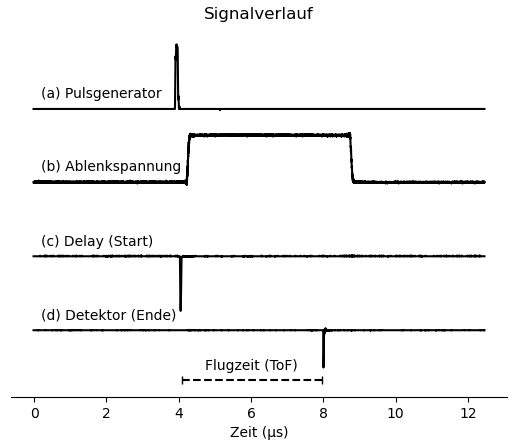
\includegraphics[width=.9\textwidth]{Signalverlauf.png}
    \caption[Aufgenommenener Verlauf der relevanten Signale der ToF-Messung]{Aufgenommenener Verlauf der relevanten Signale. (a) zeigt den initialen Spannungspuls aus dem Pulsgenerator, mit dem auch die Elektronenkanone getriggert wird. Über einen Delay-Generator wird das verspätete Signal (c) erzeugt, um die Ablenkspannung (b) anzusteuern. (d) zeigt das Signal, welches auf der Anode des Detektors entsteht, nachdem es durch den CFD gelaufen ist. Die zeitliche Differenz aus (c) und (d) entspricht der Flugzeit}
    \label{fig:Signal} 
\end{figure}

\subsection{Positionssensitive Auflösung}
In Abbildung \ref{fig:pos} ist der Signalfluß der positionssensitiven Messung schematisch abgebildet und wird nun beschrieben. Die auf dem Drahtgitter entstandenden Signale werden mittels eines Verstärkers von Roentdek verstärkt, wobei darauf geachtet werden muss, dass die Pulse nicht den Verstärker sättigen. Haben die Ionen eine zu große Energie, verliert die Messung der Position an Genauigkeit. Wie auch bei der Verarbeitung der Signale für die Flugzeitmessung wird ein CFD verwendet, um den Zeitpunkt der Signale zu bestimmen. Die analoge Ausgabe des CFD wird dann einem ADC übergeben, der ausgestattet mit der Elektronik die Signale digitalisiert und für die Auswertung am Computer präpariert. Am Computer kann dann das Programm \textsc{Cobold} verwendet werden, um die von der Hardware ausgelesenen Daten zu visualisieren und zu analysieren. Da die Positionsinformationen nur für die Validierung der Messung verwendet werden, wird auf eine detaillierte Beschreibung der Verarbeitung verzichtet.

\begin{figure}
    \centering
    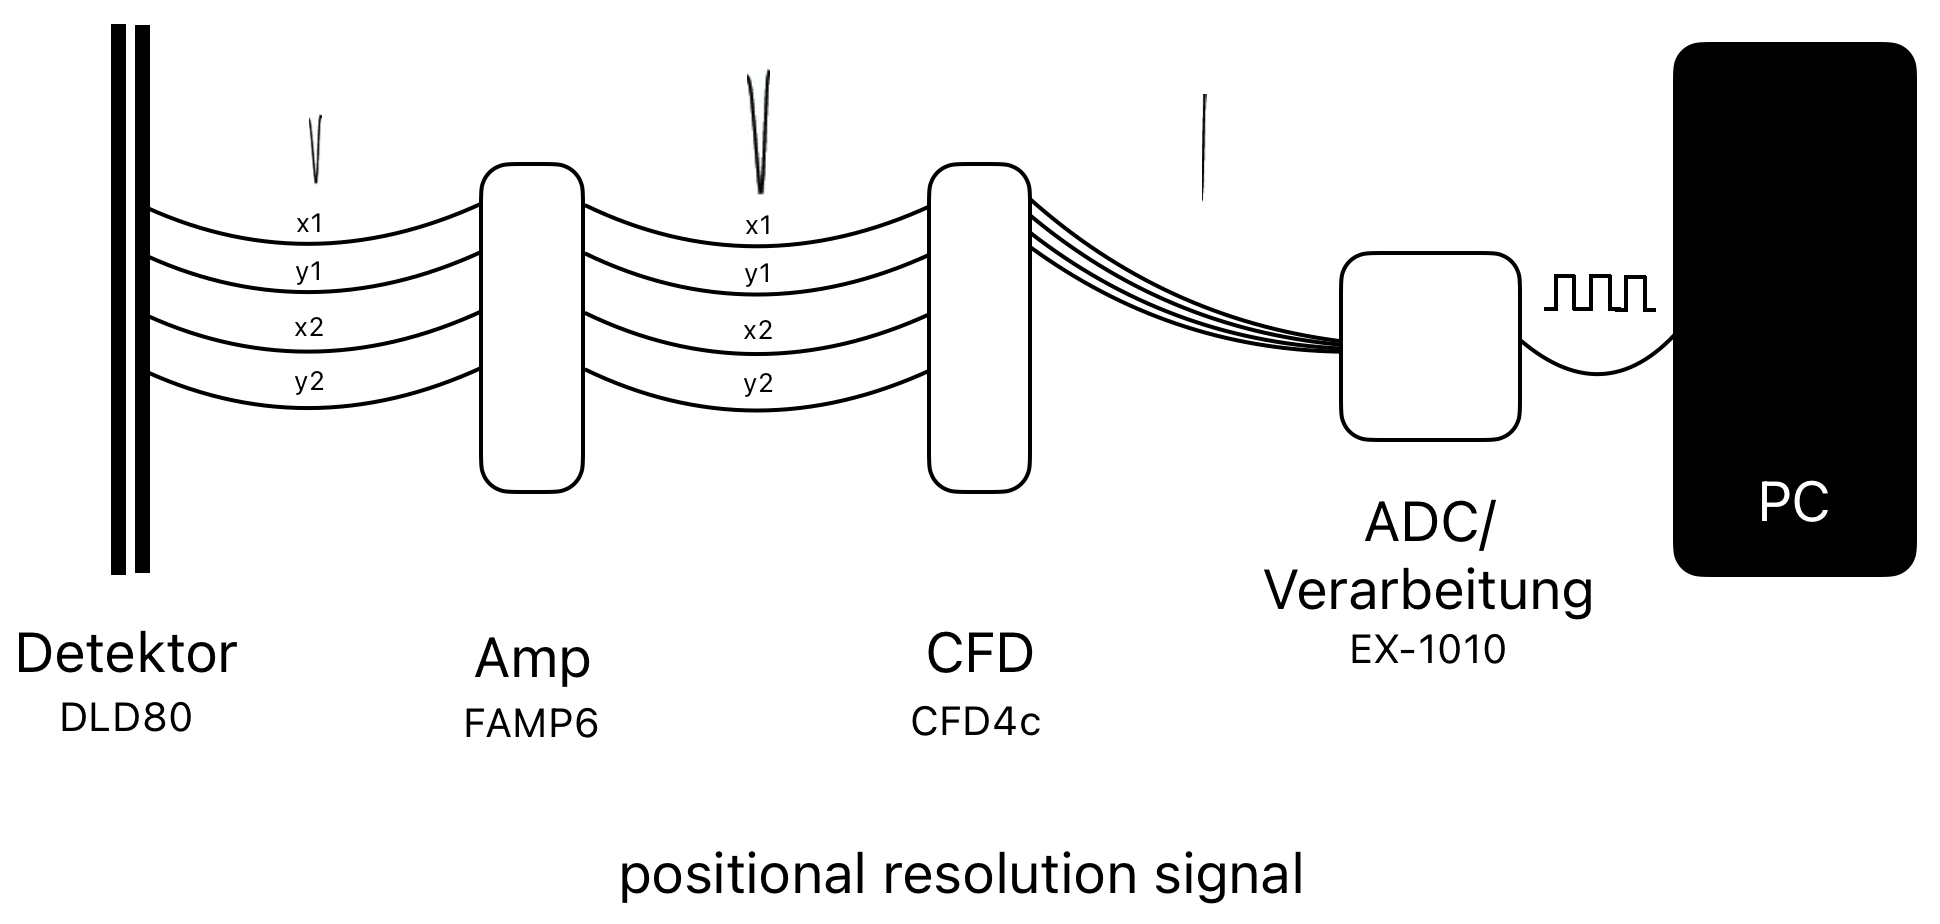
\includegraphics[width=.8\textwidth]{PosSig.png}
    \caption[Signalfluß für die positionssensitive Messung]{Schmatisch dargestellter Signalfluß für die positionssensitive Messung. Die Positionsdaten werden über die Drahtgitter am Detektor erzeugt und über einen Verstärker, CFD und ADC digitalisiert. Die Daten werden dann am Computer ausgewertet.}
    \label{fig:pos} 
\end{figure}
\cleardoublepage
\chapter{Auswertung}
\label{chap:Auswertung}
In diesem Kapitel sollen die im Experiment gewonnen Messdaten ausgewertet werden. Bereits bei einer Kalibrationsmessreihe mit Argon konnten aufgrund einer Fehlfunktion der Elektronenkanone keine vollständigen Wirkungsquerschnitte aufgenommen werden. Die Zahl der Elektronen, die für die Berechnung des Wirkungsquerschnittes benötigt werden, kann nicht ausreichend genau eingestellt werden, sodass gerade bei geringeren Energien keine Messung möglich ist. Nach einer Reperatur sollte dies wieder möglich sein. 

Aus diesem Grund kann nur eine qualitative Auswertung einer Kalibrationsmessung mit Argon, sowie eines Restgasspektrums durchgeführt werden. Anschließend folgt eine Simulation der Ionenoptik des Massenspektrometers, mit der alternativ die Genauigkeit des Massenspektrometers überprüft werden kann.

\section{Kalibrationsmessung mit Argon}
Um die Anlage mit einem bereits gut untersuchten Gas zu Testen, wurde eine Testreihe mit Argon durchgeführt. Da es bereits Probleme mit der Bestimmung der Elektronenzahl aufgrund einer Fehlfunktion der Kanone gab, können nur qualitative Aussagen getroffen werden. Ein besonders kleiner Extraktionsstrom der Kanone bei niedrigen Eletrkonenenergien macht eine Messung des Elektronenstroms zu ungenau. Die Bestimmung der Ionisierungsquerschnitt ist nicht möglich, da die Elektronenzahl direkt in die Formel eingeht, es können jedoch qualitative Aussagen über die relativen Häufigkeiten der Ionen getroffen werden, welche propotional zum Ionisierungsquerschnitt sind.

Die Auswertung der Messdaten erfolgt über einen digitalen Vielkanalanalysator (engl. \textit{multi channel analyzer}, MCA), der auf einem Computer Histogramme der aus der Flugzeit generieten Pulshöhen erstellt. Der MCA hat 4096 diskreten Kanäle, welche den Zeitbereich von 0 bis zur maximalen Zeit des TPHC abdecken. Diese werden dann mit Python und \textit{Matplotlib}, \textit{SciPy} und \textit{numpy} weiter ausgewertet und dargestellt. 

\begin{figure}
    \centering
    \hspace{-1.6cm}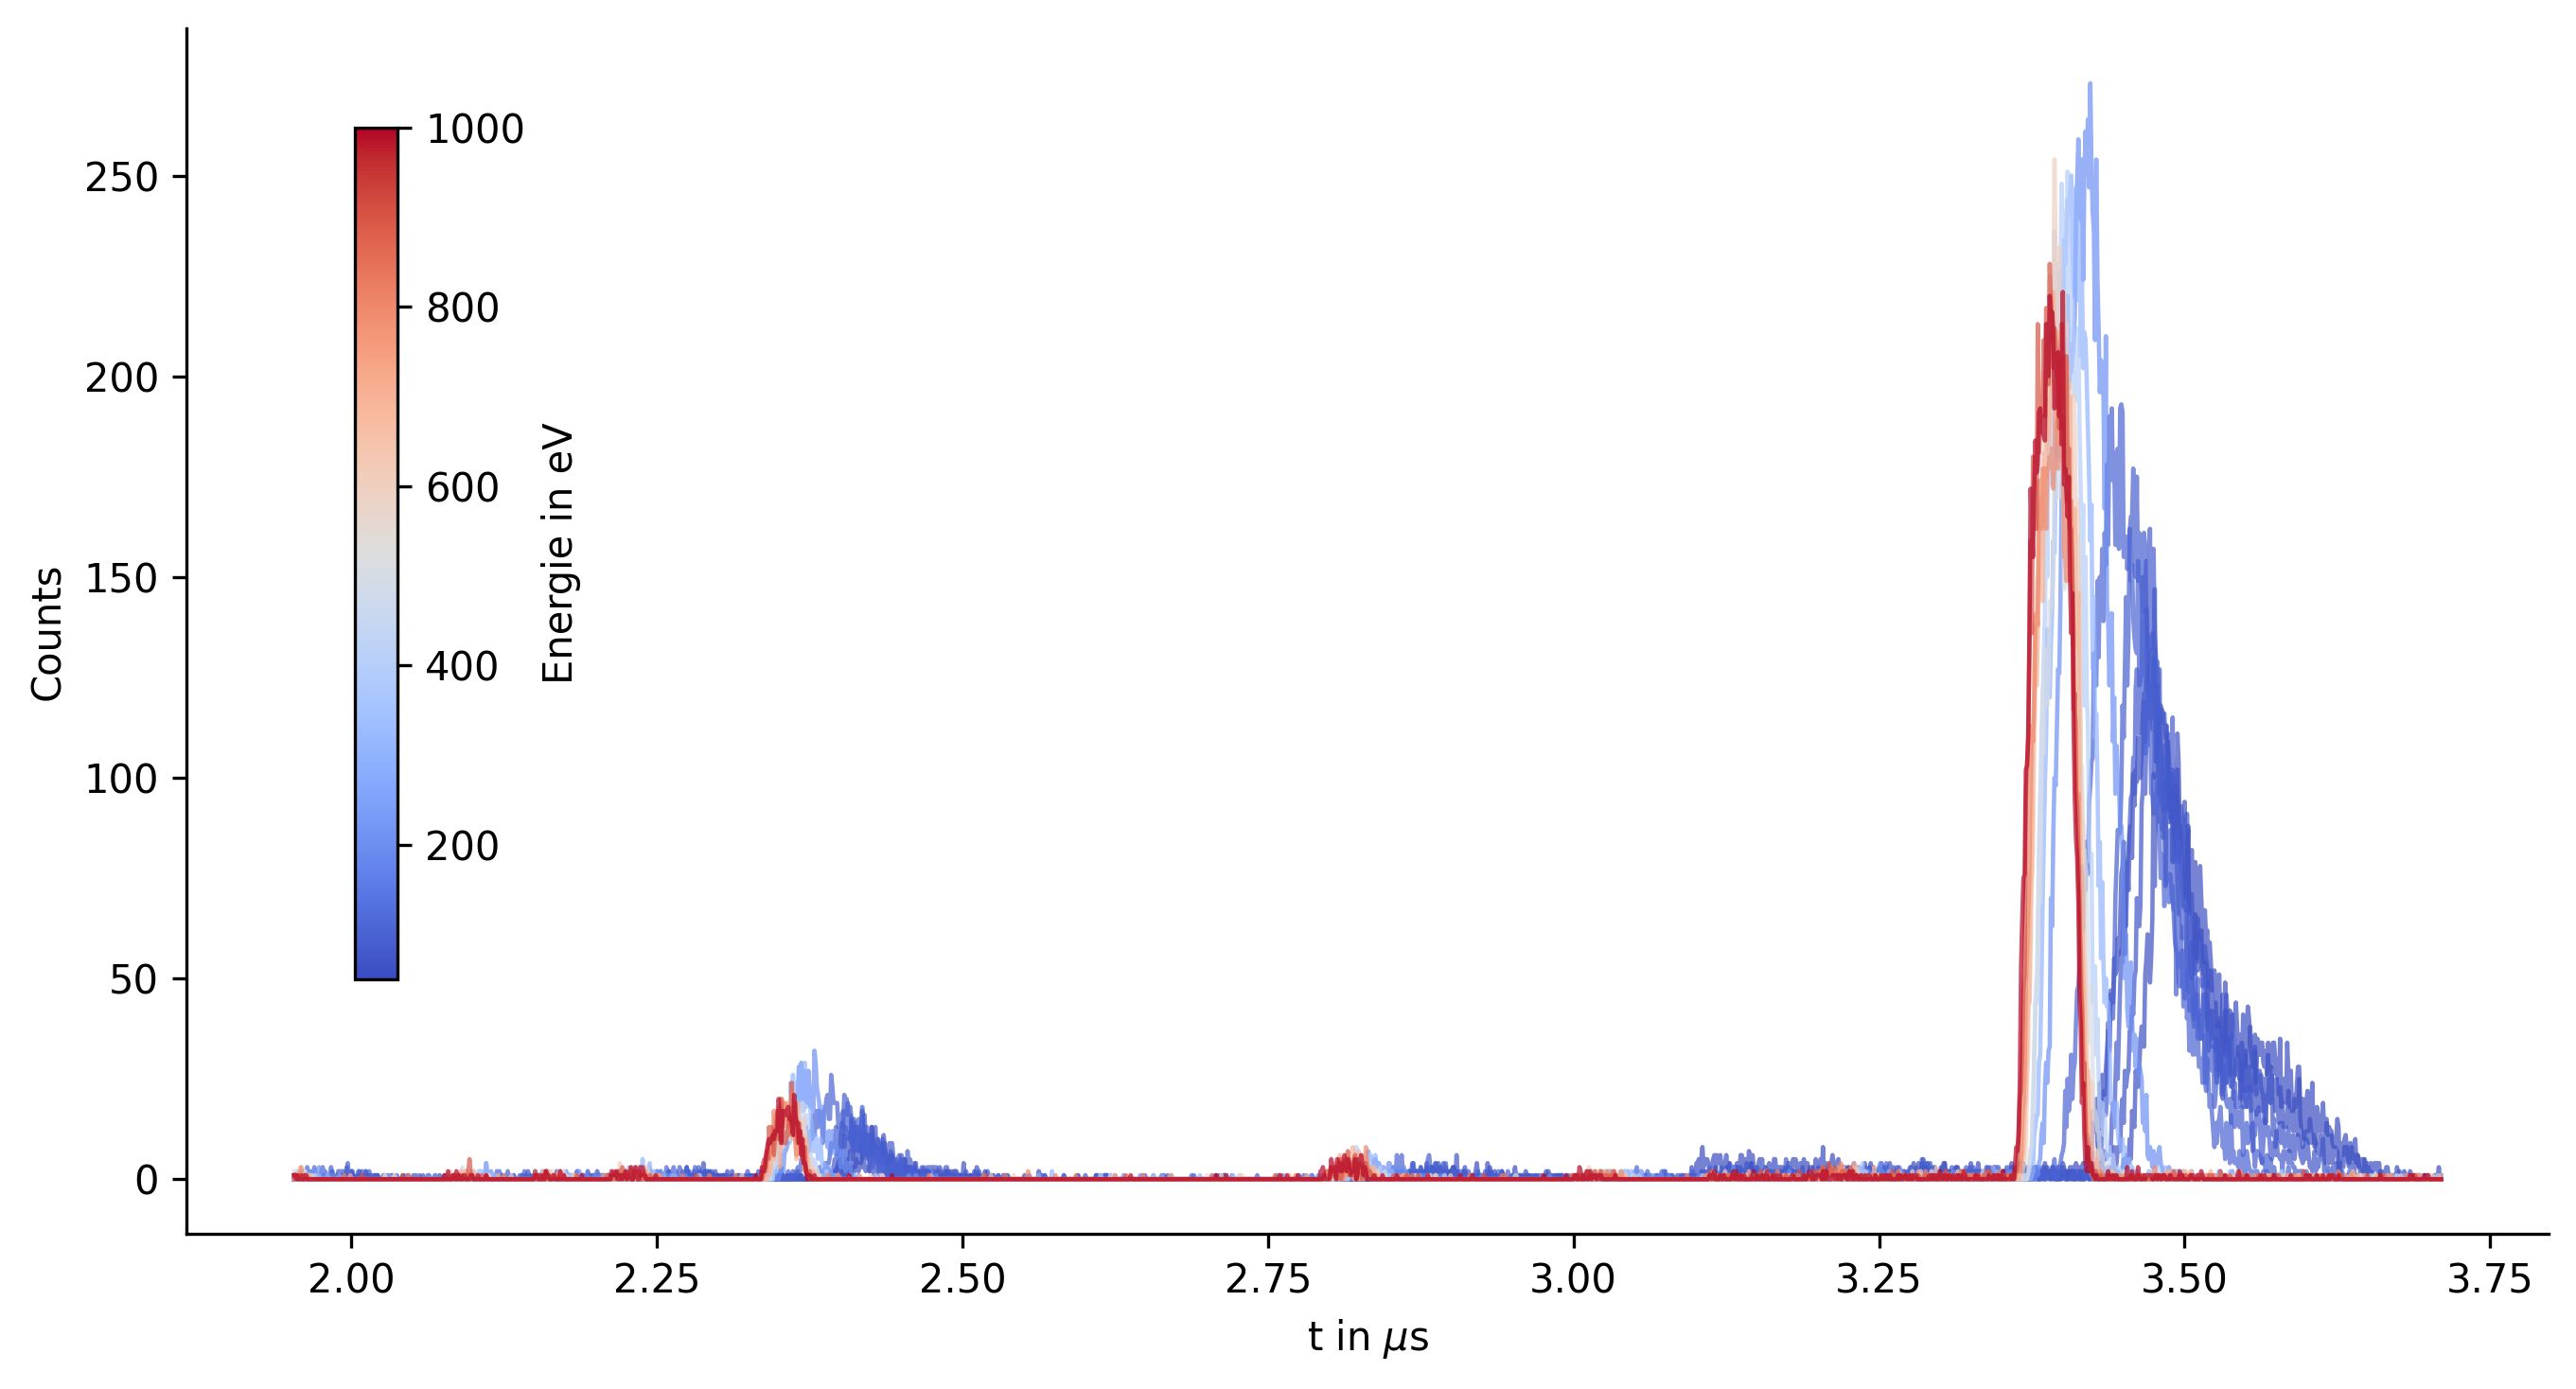
\includegraphics[width=1.1\textwidth]{Ar50-1000eV.png}
    \caption[Flugzeitspektrum von Argon bei Elektronenenergie von 50 bis 1000 eV]{Flugzeitspektrum von Argon bei Elektronenenergie von 50 bis 1000 eV. Die Messungen sind jeweils über 60 Sekunden entstanden.}
    \label{fig:ar}
\end{figure}

Abbildung \ref{fig:ar} zeigt unskalierte Flugzeitspektren von Argon bei Elektronenenergien von 50 bis 1000 eV. Es ist zu erkennen, dass die Peaks mit steigender Elektronenenergie schärfer werden und es einen Zusammenhang zwischen der Elektronenenergie und der Flugzeit gibt, der im Folgenden genauer untersucht wird. Dass die Peaks schärfer werden ist unter anderem darauf zurückzuführen, dass die Elektronenkanone bei höheren Energien einen schärferen Strahl erzeugt. Die thermische Bewegung der Elektronen hat weniger Einfluss gegenüber der deutlich höheren kinetischen Energie. Der Entstehungsort der Ionen ist dann genauer definiert, was zu schmaleren Peaks führt.

\subsection{Zusammenhang von Flugzeit und Elektronenenergie}
Woher genau dieser Zusammenhang kommt, kann nicht direkt aus den Daten abgeleitet werden, da ein höherer Energieübertrag auf die Gasatome nicht direkt die Flugzeit beeinflussen kann. Es kann aber vermutet werden, dass dieses Phänomen mit der verzögerten Extraktion der Ionen aus dem Kondensator zusammenhängt, die Ionen mit höheren kinetischen Energien schneller beschleunigt. Genauere Untersuchungen folgen in Kapitel \ref{sec:delay} zur Simulation. Anhand der mittleren Flugzeit des größten Peaks der verschiedenen Spektren kann der Zusammenhang zwischen der Elektronenenergie und der Flugzeit untersucht werden.
Abbildung \ref{fig:tof_energy} zeigt die Flugzeit des größten Peaks in Abhängigkeit der Elektronenenergie. Es ist zu erkennen, dass die Flugzeit mit steigender Elektronenenergie $E$ sinkt. Ein Fit der Form $t = a\sqrt{E} + b$ zeigt, dass die Flugzeit propotional zu $\sqrt{E}$ ist.

\begin{figure}
    \centering
    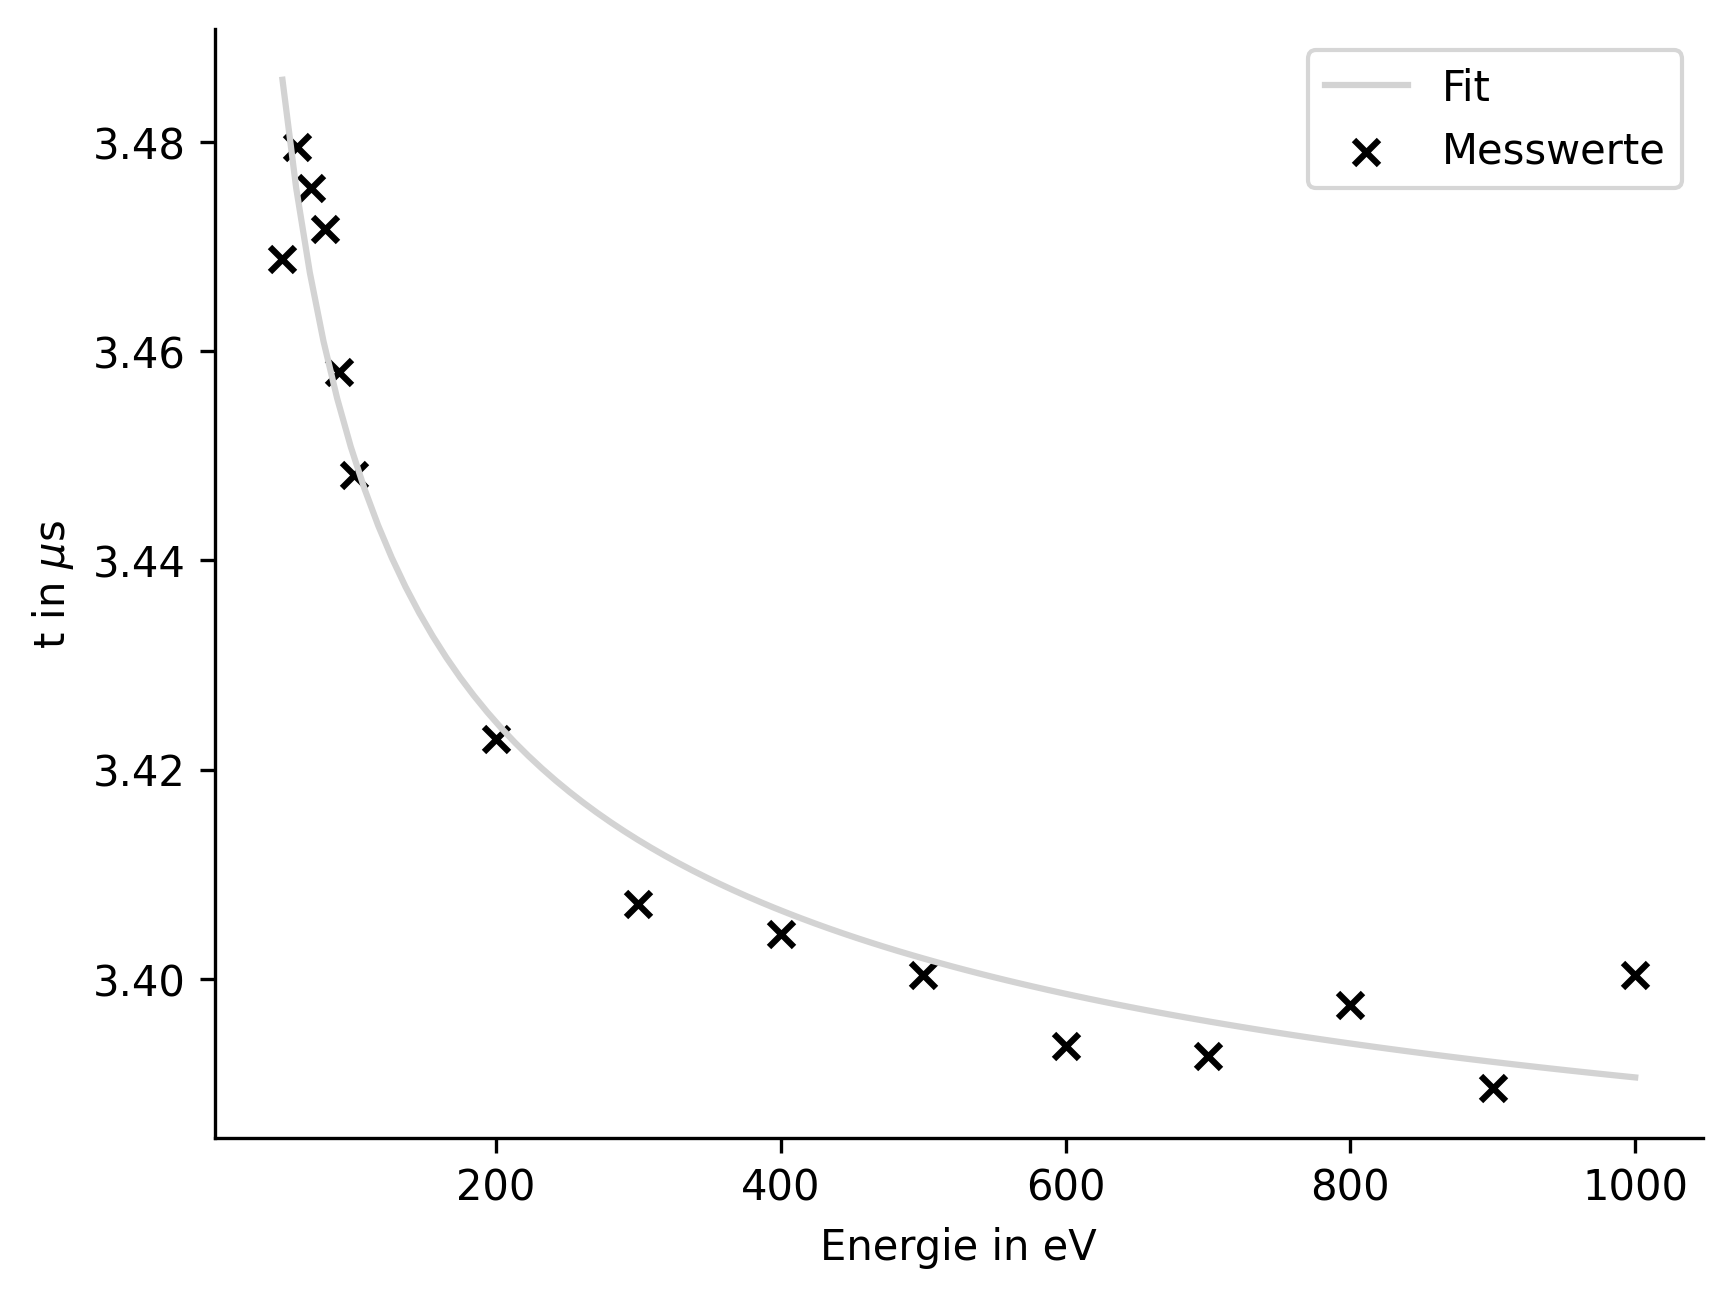
\includegraphics[width=.7\textwidth]{tof_energy.png}
    \caption[Zusammenhang zwischen TOF und Elektronenenergie]{Abbildung der Flugzeit des größten Peaks in Abhängigkeit der Elektronenenergie. Ein Fit zeigt, dass eine Funktion der Form $t = a\sqrt{E} + b$ den Zusammenhang gut beschreibt.}
    \label{fig:tof_energy}
\end{figure}

\subsection{Transformation in ein Massenspektrum}
Für eine weitere Analyse muss das Flugzeitspektrum in ein Massenspektrum transformiert werden. Um das Spektrum korrekt skalieren zu können, werden die Peaks mit einem Referenzspektrum verglichen und einzelne identifiziert. Im Fall der Kalibrationsmessung mit Argon wurde ein Spektrum von Straub \textit{et al.} \cite{Straub} als Vergleich verwendet, bei dem die Peaks von ein- bis vierfach geladenen Argonionen identifiziert wurden. Anhand dieser Information kann das Spektrum skaliert werden, um die Masse-zu-Ladungsverhältnisse auf der horizontalen Achse zu erhalten. Die Transformationsfunktion hat die Form $at^2+b$, wobei die Parameter über die Zuordnung des Masse-zu-Ladungsverhältnisses von mindestens drei Punkten ermittelt werden können. Diese Form beschreibt die Abhängigkeit des Masse-zu-Ladungsverhältnisses von der Flugzeit hinreichend gut, da die gesamte Flugzeit nach Gleichung \ref{eq:time} propotional zu $\sqrt{m/q}$ ist. Zusätzlich kann mit einem zweiten Parameter ein Offset eingestellt werden, der durch Einstellungen am ADC entstehen kann. 

Um einen Vergleich mehrerer Spektren zu ermöglichen, werden die Spektren zunächst normalisiert. Das bedeutet, dass die Fläche des größten Peaks (Ar$^+$) auf 1 gesetzt wird. Da sich der Ionisationsquerschnitt mit der Elektronenenergie ändert, werden die Spektren anschließend mit den Werten für $\sigma^+$ gewichtet. Der Count der Ionen geht direkt proportional in den Ionisierungsquerschnitt $\sigma^+$ ein. Tabelle \ref{tab:argon} zeigt einen Auszug der Ionisierungsquerschnitte von Argon aus \cite{Straub}.

\subsection{Unsicherheiten}
Durch die begrenzte Zahl der Kanäle des MCA ergibt sich eine Unsicherheit \begin{equation}
    \Delta t_{\text{MCA}} = \frac{4 \text{ $\mu$s}}{4096} = 0.977 \text{ ns},
\end{equation} 
die sich auf eine Masseunsicherheit umrechnen lässt. Dafür muss die Fehlerfortpflanzung der Transformationsfunktion berücksichtigt werden:
\begin{equation}
    \Delta m/q = \sqrt{\left(\frac{\partial f_{Trans}}{\partial t}\right)^2 \Delta t_{\text{MCA}}^2} = 2at\Delta t_{\text{MCA}}.
\end{equation}
$a$ ist dabei der erste Parameter der Transformationsfunktion $f_{Trans}$, der bei einer Elektronenerngie von 100 eV bei einem Argonspektrum 3.02$\times 10^{-6}$ beträgt. Bei einer Flugzeit von 3.5 $\mu$s beträgt dann die Unsicherheit der Masse 0.129 u/e. Das bedeutet, dass eine Masse von 40 u/e mit einer Unsicherheit von 0.129 u/e gemessen wird. Die Auflösung in der Realität kleiner, da die Peaks nicht unendlich schmal sind und sich über mehrere Kanäle erstrecken.

\subsection{Extraktionverzögerung}
Die Verzögerung der Extraktion bei der DETOF-Methode ermöglicht schärfere Flugzeitpeaks. Für die bisherige Auswertung wurde eine tatsächliche Extraktionsverzögerung von etwa 300 ns verwendet. Das geht aus den Signalen hervor (Abbildung \ref{fig:Signal}). Besonderns bei niedrigen Energien sind die Peaks sehr breit und unsymmetrisch. Eine Verdopplung der Extraktionszeit auf 600 ns macht die Peaks deutlich schärfer und verbessert so auch die darstellbare Auflösung. Abbildung \ref{fig:delay} zeigt die Flugzeitspektren von Argon bei 50 eV mit einer Extraktionsverzögerung von 300 ns und 600 ns. Eine weitere Verlängerung der Extraktionsverzögerung hat nicht den selben Effekt. Aufgrund der deutlichen Verbesserung sind folgende Spektren mit 600 ns Verzögerung aufgenommen worden.
\begin{figure}
    \centering
    \begin{subfigure}{.45\textwidth}
        \centering
        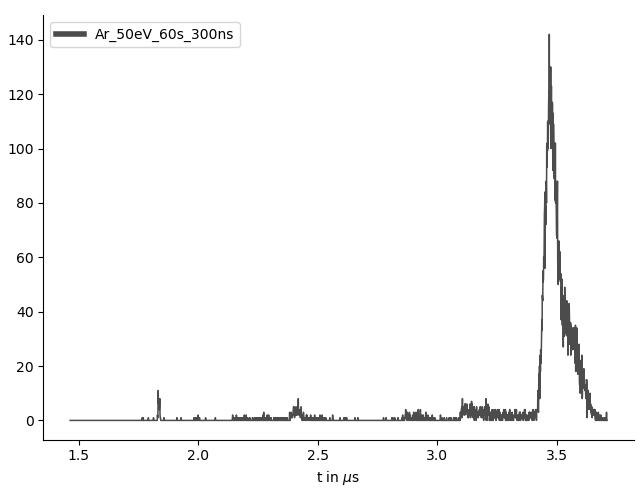
\includegraphics[width=1\linewidth]{Ar50-300ns.png}
        \caption{Argon bei 50 eV mit 300 ns Extraktionsverzögerung}
    \end{subfigure}%
    \hfill
    \begin{subfigure}{.45\textwidth}
        \centering
        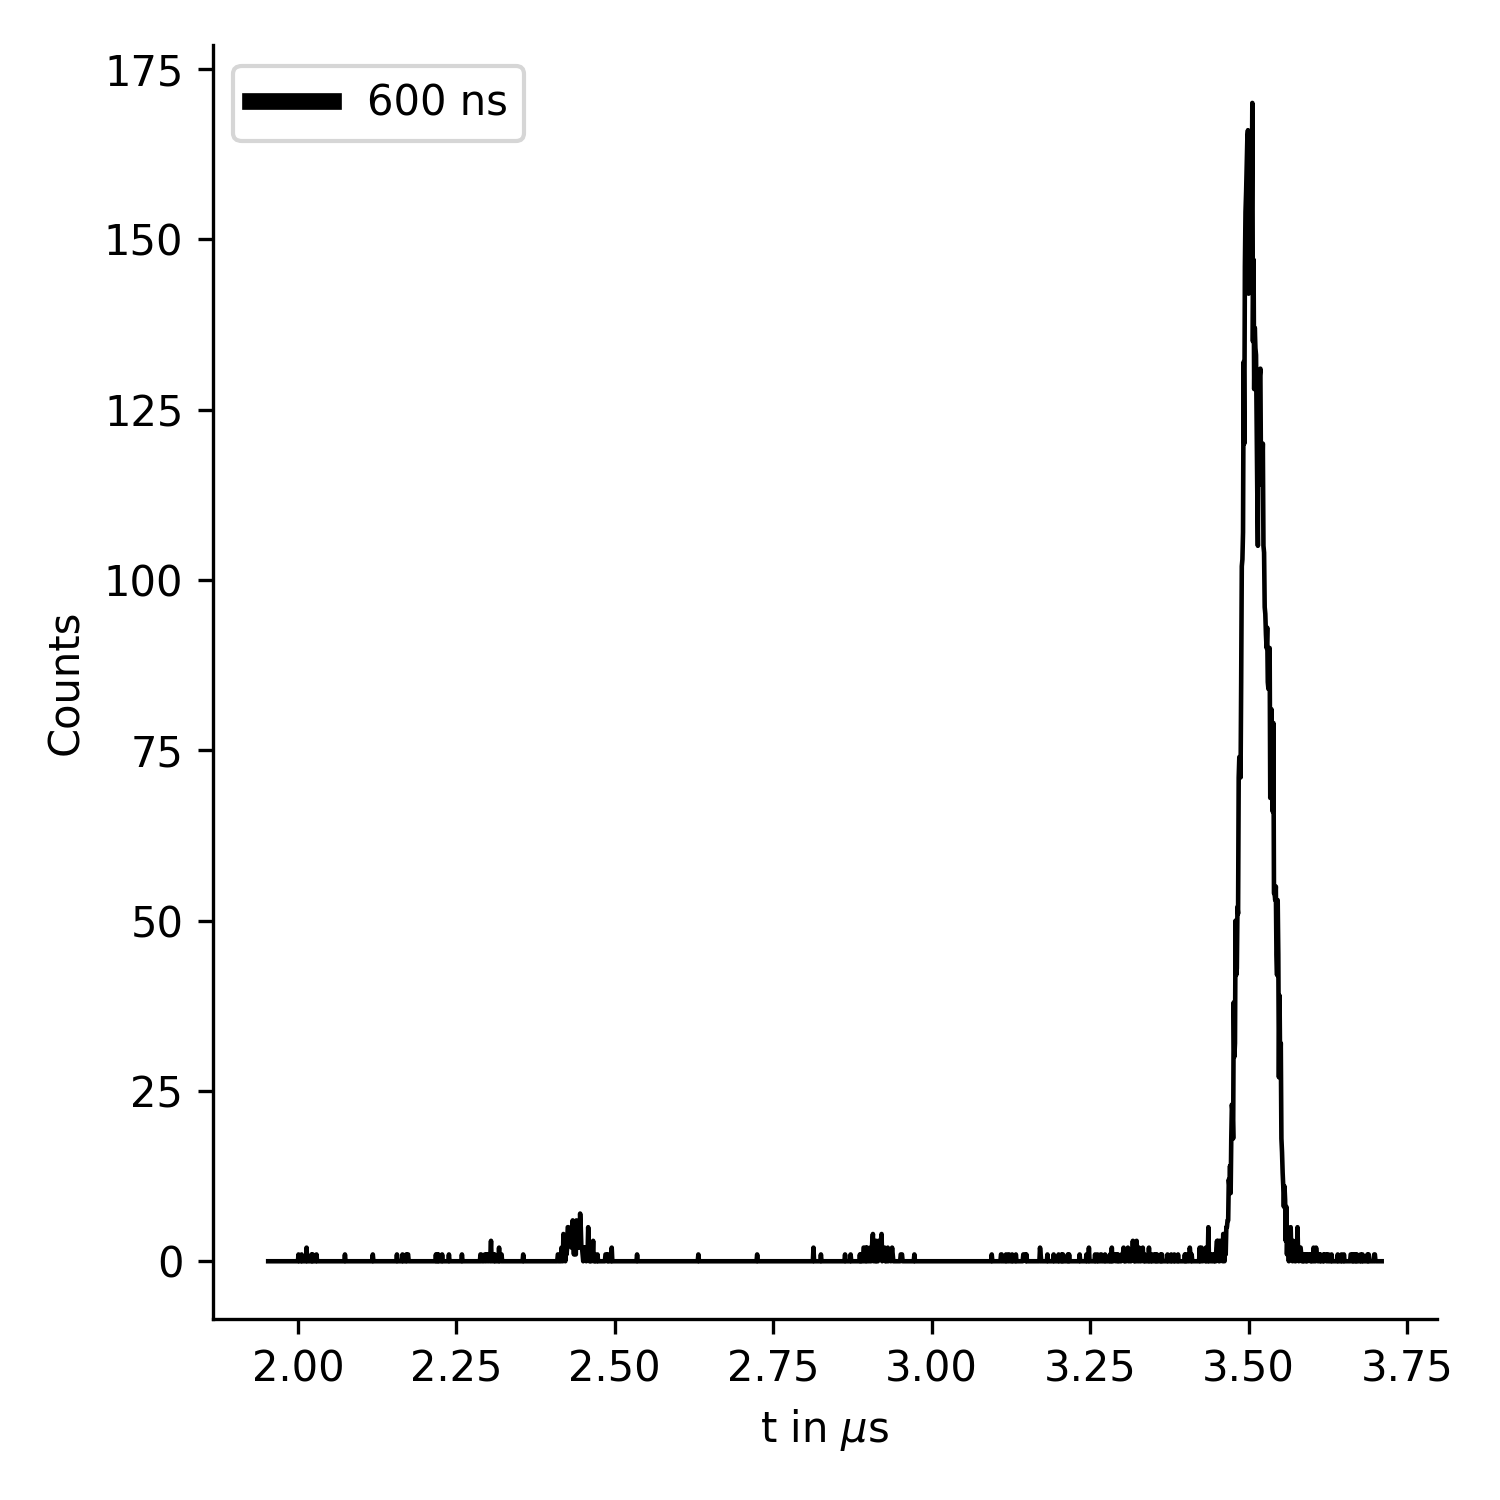
\includegraphics[width=1\linewidth]{Ar50-600ns.png}
        \caption{Argon bei 50 eV mit 600 ns Extraktionsverzögerung}
        
    \end{subfigure}
    \caption{Flugzeitspektren von Argon bei 50 eV mit unterschiedlichen Extraktionsverzögerungen.}
    \label{fig:delay}
\end{figure}

\subsection{Analyse und Vergleich der Ergebnisse}
Abbildung \ref{fig:ar_scaled} zeigt das Spektrum aus Abbildung \ref{fig:ar} nach Anwendung der Transformationsfunktion und Normalisierung. Die Peaks der ein- bis vierfach geladenen Argonionen sind in den Spektren gut zu erkennen. Außerdem sind einige weitere Peaks mit Fragmenten von Wasser, Kohlenstoff und atmosphärischen Gasen sichtbar. Diese werden im nächsten Abschnitt besprochen. Die Spektren zeigen auch, dass erst beim Erreichen einer bestimmten Elektronennergie Mehrfachionisationprozesse stattfinden können. Die Wirkungsquerschnitte für die Mehrfachionisationen sind zwar deutlich kleiner als für die DI, dennoch nimmt der Anteil der DI als Folge mit steigender Elektronenerngie ab. Dass dieser Effekt sichtbar ist, zeigt, dass die Ionisation in der Anlage erfolgreich unter Einzelstoßbedingungen stattfindet. 


\begin{landscape}
    \begin{figure}
        \centering
        \hspace*{-3cm}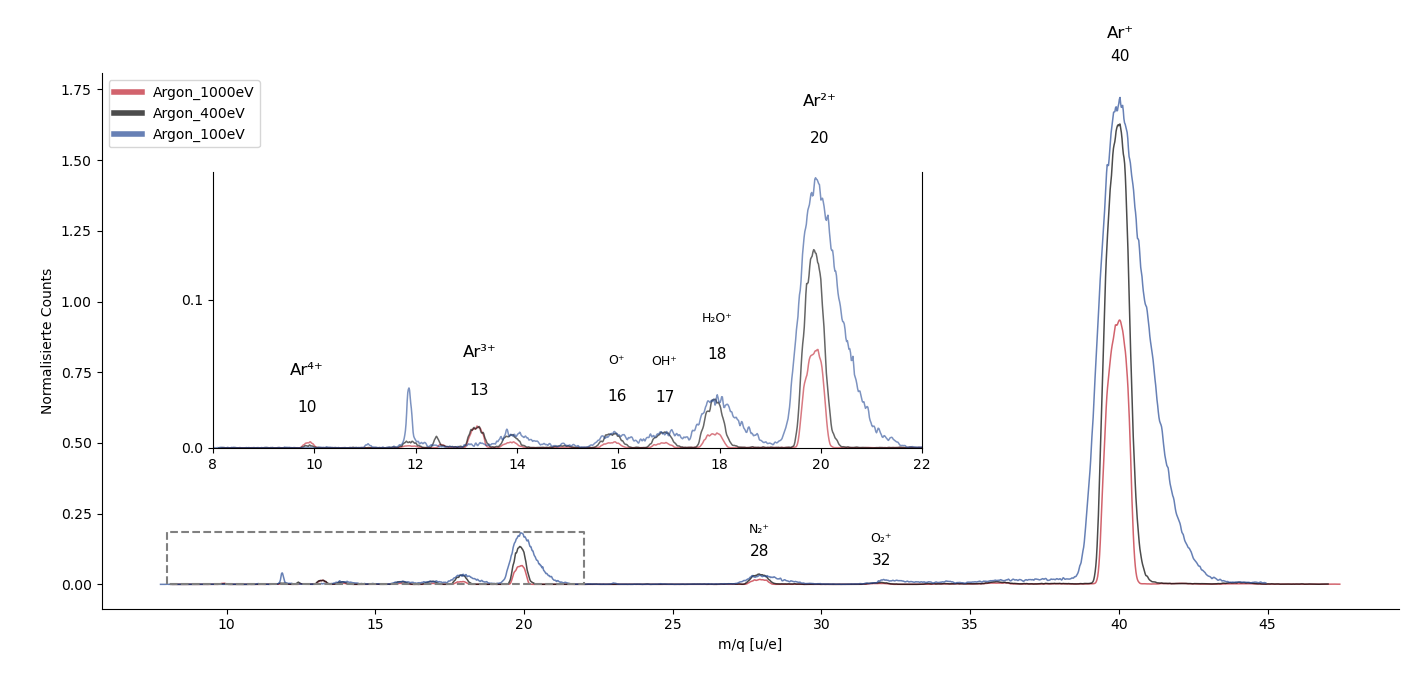
\includegraphics[width=1.7\textwidth]{Ar_scaled.png}
        \caption[Skaliertes Massenspektrum von Argon bei verschiedenen Elektronenenergien]{Masse-zu-Ladungsspektrum von Argon bei Elektronenenergien von 100, 400 und 1000 eV. Die Messungen sind jeweils über 30 Minuten entstanden. Die Spektren wurden normarlisiert und sind mit den Werten aus \ref{tab:argon} gewichtet dargestellt. Außerdem wurden sie mit einem gauß'schen 1D-Filter ($\sigma = 1$) leicht geglättet, um sie besser vergleichen zu können.}
        \label{fig:ar_scaled}
    \end{figure}
\end{landscape}

Obwohl die Werte für die Ionisierungsquerschnitte aufgrund der defekten Kanone nicht direkt ermittelt werden können, soll anhand der relativen Häufigkeiten der Ionen eine qualitative Aussage über die relativen Ionisierungsquerschnitte getroffen werden. Das bedeutet, dass das Verhältnis $\sigma^+$/$\sigma^{2+}$ dem Verhältnis der Flächen $A(\text{Ar}^+)$/$A(\text{Ar}^{2+})$ entsprechen sollte. Dies kann mit einem direkten Vergleich  mit den Werten aus \ref{tab:argon} überprüft werden. Abbildung \ref{fig:ar_ratio} zeigt die Grenzen der Integration und die Bestimmung der Verhältnisse. Für einen einfachen Vergleich wurde die Fläche des Ar$^+$-Peaks auf 0.795 gesetzt, dem entsprechenden Quersschnitt aus Tab. \ref{tab:argon}. In Tabelle \ref{tab:vergleich} sind die normierten Werte der Ionen und die prozentualen Abweichungen zu den Werten von Straub \textit{et al.} \cite{Straub} angegeben. Es ist zu erkennen, dass die Werte für die ein- und zweifach geladenen Ionen besser übereinstimmen, während die Werte für die dreifach und vierfach geladenen Ionen größere prozentuale Abweichungen haben. Dies ist vermutlich auf die geringe Anzahl an Ionen zurückzuführen, die bei höheren Energien entstehen. Insgesamt zeigt die qualitative Auswertung, dass die Anlage erfolgreich arbeitet, da die relativen Häufigkeiten der Ionen den Erwartungen in etwa entsprechen. 

\begin{figure}
    \centering
    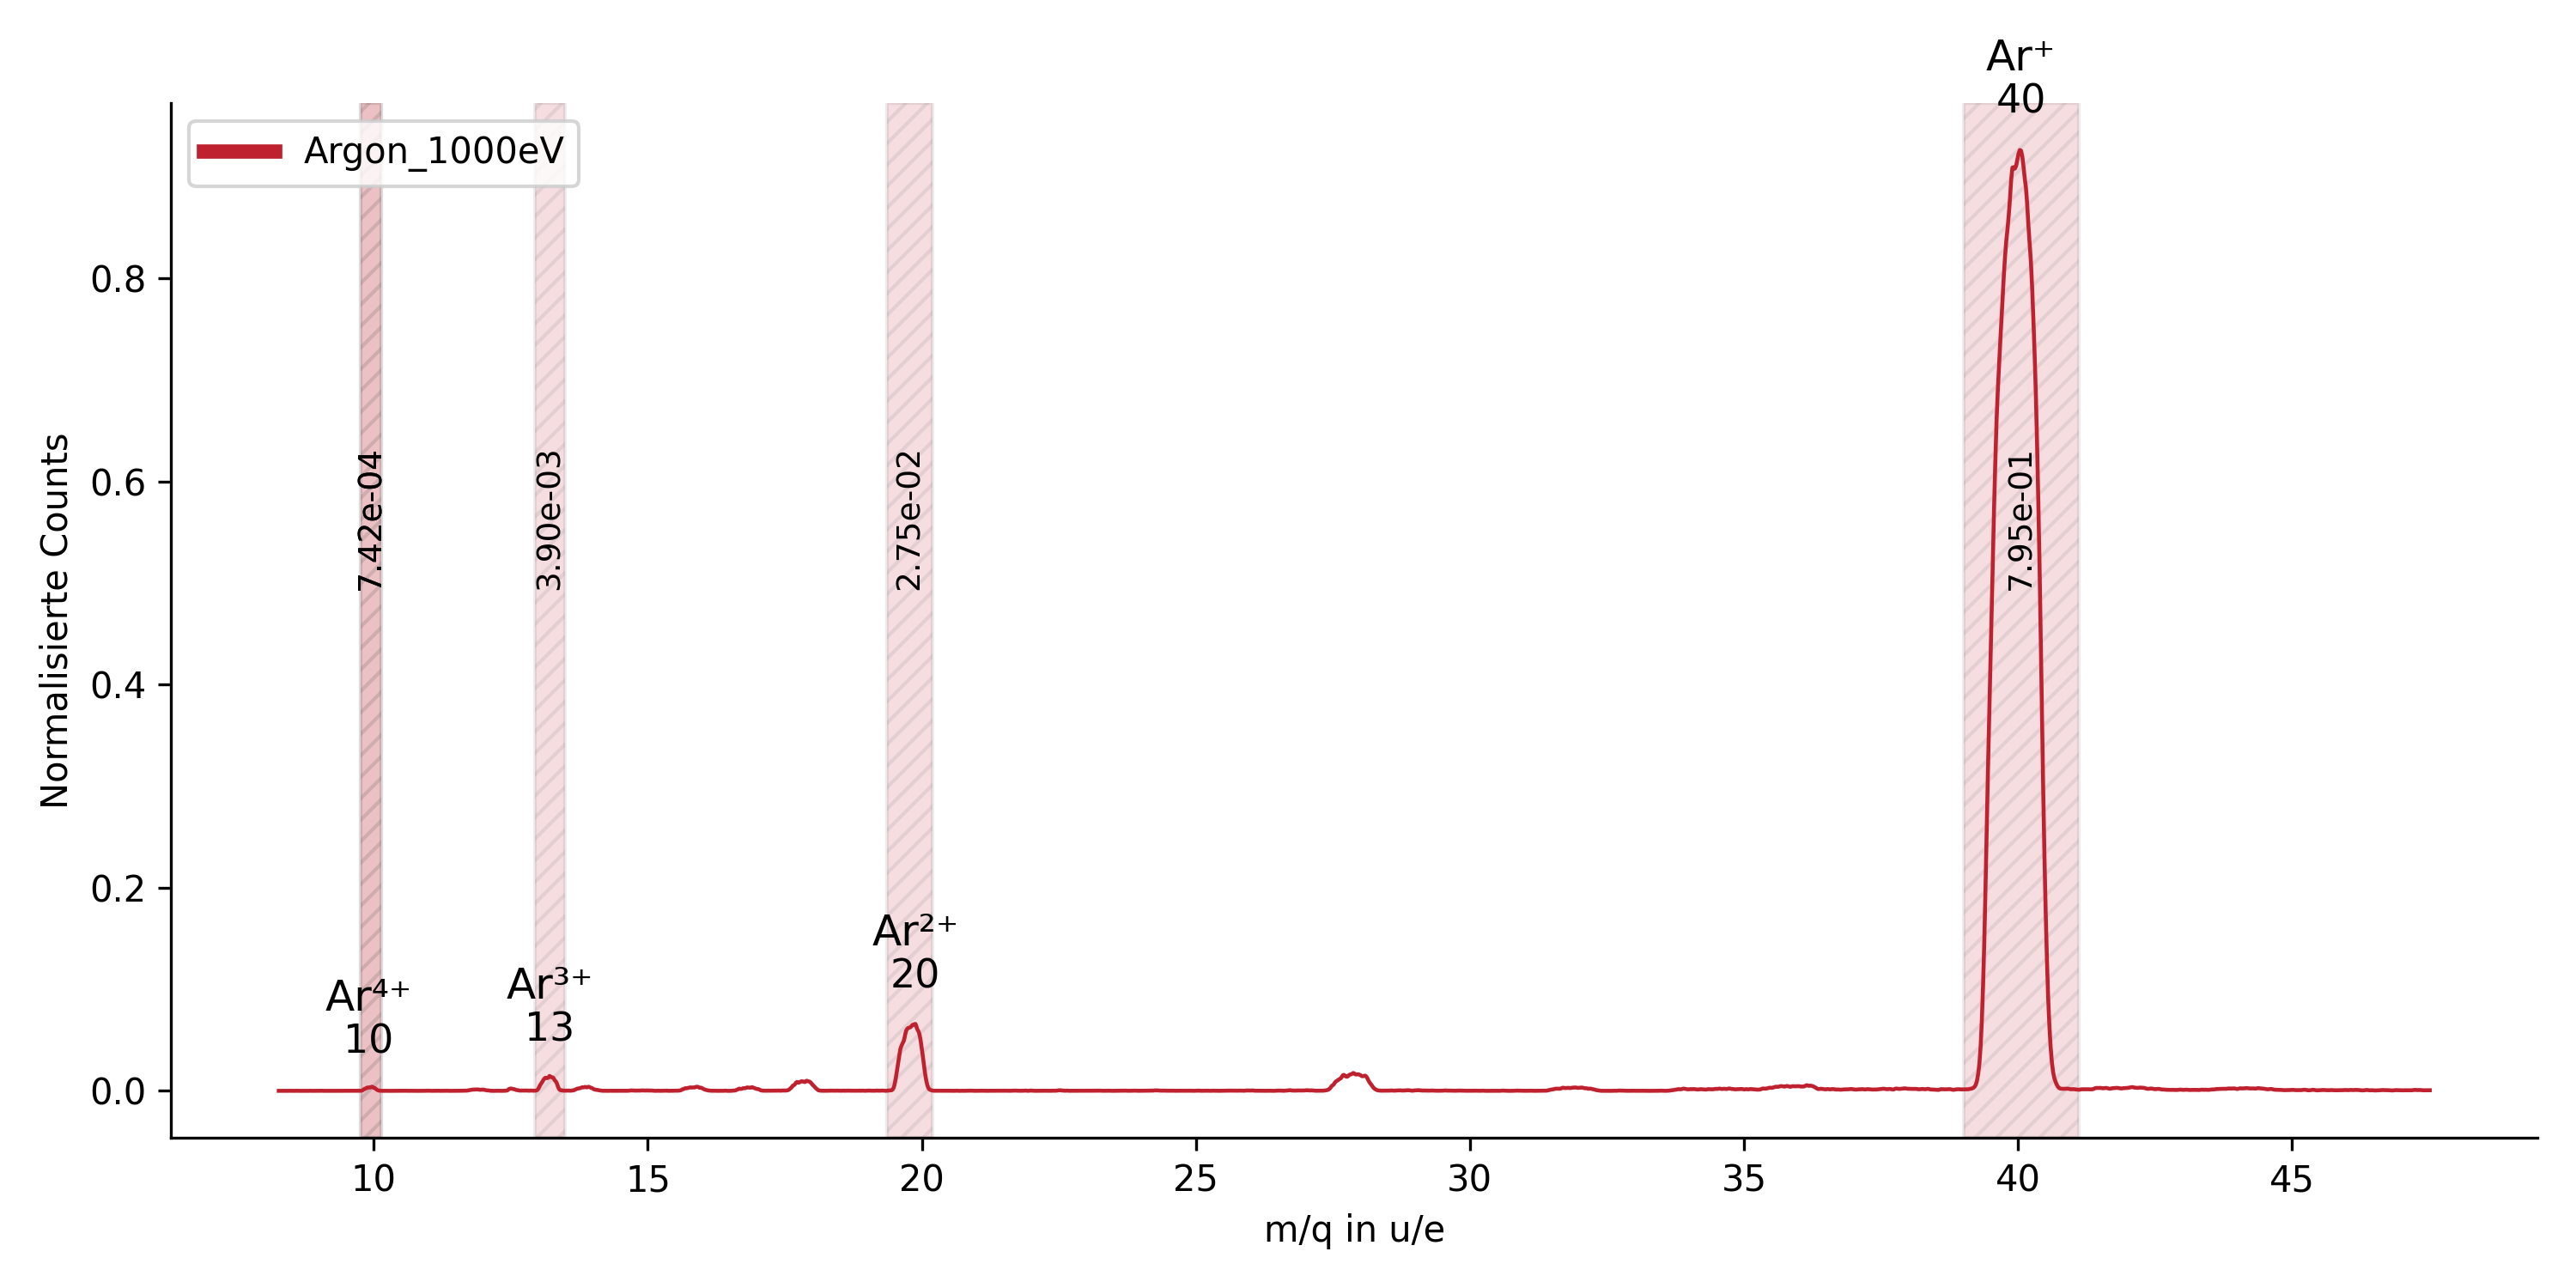
\includegraphics[width=1\textwidth]{Ar_integrated.png}
    \caption[Integration eines gewichteten Argonspektrums bei 1000 eV]{Integration eines gewichteten Argonspektrums bei 1000 eV.}
    \label{fig:ar_ratio}
\end{figure}

\begin{table}
    \centering
    \caption[Auszug der Ionisierungsquerschnitte von Argon aus Straub \textit{et al.} \cite{Straub}]{Auszug der Ionisierungsquerschnitte von Argon aus Straub \textit{et al.} \cite{Straub}. Beim Summieren der einzelnen Querschnitte zum totalen Querschnitt werden die Werte entsprechend der Ladung gewichtet:
    $\sigma^{\text{total}} = \sigma^+ + 2\sigma^{2+} + 3\sigma^{3+} + 4\sigma^{4+}$.}
    \label{tab:argon}
    \begin{tabular}{r c c c c c}
        \toprule
        \textbf{Energie} & $\sigma^+$ & $\sigma^{2+}$ & $\sigma^{3+}$ & $\sigma^{4+}$ & $\sigma^{\text{total}}$ \\
        (eV) & ($10^{-16}$ cm$^2$) & ($10^{-17}$ cm$^2$) & ($10^{-19}$ cm$^2$) & ($10^{-19}$ cm$^2$) & ($10^{-16}$ cm$^2$) \\
        \midrule
        %17  & 0.017  &        &        &        & 0.017  \\
        %20  & 0.46   &        &        &        & 0.46   \\
        %25  & 1.24   &        &        &        & 1.24   \\
        %30  & 1.84   &        &        &        & 1.84   \\
        %35  & 2.26   &        &        &        & 2.26   \\
        %40  & 2.55   &        &        &        & 2.55   \\
        %45  & 2.66   & 0.0048 &        &        & 2.66   \\
        50  & 2.70   & 0.128  &        &        & 2.73   \\
        %55  & 2.69   & 0.418  &        &        & 2.77   \\
        %60  & 2.67   & 0.856  &        &        & 2.84   \\
        %65  & 2.67   & 1.21   &        &        & 2.91   \\
        %70  & 2.67   & 1.46   &        &        & 2.96   \\
        %75  & 2.66   & 1.56   &        &        & 2.97   \\
        %80  & 2.69   & 1.70   &        &        & 3.03   \\
        %85  & 2.70   & 1.79   &        &        & 3.06   \\
        %90  & 2.69   & 1.84   &        &        & 3.06   \\
        %95  & 2.67   & 1.90   & 0.51   &        & 3.05   \\
        100 & 2.64   & 1.89   & 1.03   &        & 3.02   \\
        %110 & 2.61   & 1.91   & 2.21   &        & 3.00   \\
        %120 & 2.55   & 1.87   & 3.23   &        & 2.93   \\
        %140 & 2.45   & 1.77   & 4.94   &        & 2.81   \\
        %160 & 2.35   & 1.65   & 5.57   &        & 2.70   \\
        %180 & 2.27   & 1.58   & 5.68   &        & 2.60   \\
        %200 & 2.18   & 1.44   & 5.53   &        & 2.49   \\
        %225 & 2.10   & 1.31   & 5.30   &        & 2.37   \\
        %250 & 1.99   & 1.25   & 5.23   &        & 2.25   \\
        %275 & 1.87   & 1.13   & 5.09   &        & 2.11   \\
        %300 & 1.79   & 1.08   & 5.03   &        & 2.02   \\
        %350 & 1.63   & 0.953  & 5.99   & 0.17   & 1.84   \\
        400 & 1.51   & 0.872  & 6.32   & 0.44   & 1.71   \\
        %450 & 1.39   & 0.759  & 6.50   & 0.77   & 1.57   \\
        %500 & 1.31   & 0.679  & 6.97   & 1.07   & 1.47   \\
        %550 & 1.23   & 0.623  & 7.08   & 1.18   & 1.38   \\
        %600 & 1.16   & 0.575  & 7.41   & 1.32   & 1.30   \\
        %650 & 1.09   & 0.552  & 7.19   & 1.27   & 1.23   \\
        %700 & 1.03   & 0.524  & 7.23   & 1.33   & 1.16   \\
        %750 & 0.976  & 0.496  & 6.97   & 1.42   & 1.10   \\
        %800 & 0.932  & 0.456  & 6.96   & 1.50   & 1.05   \\
        %850 & 0.901  & 0.425  & 7.09   & 1.42   & 1.01   \\
        %900 & 0.865  & 0.419  & 6.51   & 1.33   & 0.973  \\
        %950 & 0.824  & 0.394  & 6.51   & 1.36   & 0.927  \\
        1000 & 0.795 & 0.374  & 6.57   & 1.32   & 0.895  \\
        \bottomrule
    \end{tabular}
\end{table}

\begin{table}
    \centering
    \caption[Normierte Anzahl von Ionen und Abweichung zu Werten von Straub \textit{et al.}]{Normierte Anzahl von Ionen dargestellt wie in Tab. \ref{tab:argon}. In Klammern sind die prozentualen Abweichungen zu den Werten von Straub \textit{et al.} \cite{Straub} angegeben.}
    \label{tab:vergleich}
    \begin{tabular}{r c c c c c}
        \toprule
        \text{} & \multicolumn{5}{c}{\textbf{normierte Anzahl von Ionen}} \\ 

        \textbf{Energie} & $Ar^+$ & $Ar^{2+}$ & $Ar^{3+}$ & $Ar^{4+}$ & gew. Summe \\
        (eV) & (1) & ($10^{-1}$) & ($10^{-3}$) & ($10^{-3}$) & ($1$) \\
        \midrule
        50  & {2.7}  & {0.206} \textcolor{gray}{(60.9\ \%)} & {}  & {}  & {2.41} \textcolor{gray}{(11.7\ \%)}   \\
        100 & 2.64  & 1.42 \textcolor{gray}{(24.9\ \%)} & 4.04 \textcolor{gray}{(292.2\ \%)} & {} & 2.94 \textcolor{gray}{(2.6\ \%)} \\
        400 & 1.51  & 0.602 \textcolor{gray}{(31.0\ \%)} & 4.62 \textcolor{gray}{(26.9\ \%)} & 0 \textcolor{gray}{(100\ \%)} & 1.64 \textcolor{gray}{(4.1\ \%)} \\
        1000 & 0.795  & 0.278 \textcolor{gray}{(25.7\ \%)} & 3.98 \textcolor{gray}{(39.4\ \%)} & 0.763 \textcolor{gray}{(42.2\ \%)} & 0.86 \textcolor{gray}{(3.9\ \%)} \\
               
        
        \bottomrule
    \end{tabular}
\end{table}

\section{Restgasspektrum}
Eine weitere Möglichkeit zur Überprüfung des Massenspektrometers ist die Aufnahme eines Restgasspektrums. Hierbei wird kein Gas in die Kammer eingelassen und lediglich der atmosphärische Hintergrund in der Kammer gemessen. Dieser besteht aus verschiedenen Restgasen, die durch die Elektronenstoßionisation genauso ionisiert werden können. In einem Vakuum erwartet man vorallem Rückstände von Wassermolekülen, sowie stabiler Kohlenstoffverbindungen, die bei der Vakuumbildung aus den Wänden der Kammer gelöst werden, als auch Reste von Stickstoff und Sauerstoff aus der Luft. Außerdem können besonders leichte Gase, hier vorallem Wasserstoff, übrig bleiben, da sie besonders flüchtig sind und die Vakuumpumpen sie weniger effektiv entfernen können. Es ist zusätzlich praktisch die Restgasverteilung zu kennen, um sie bei der Auswertung von Messungen berücksichtigen zu können. Aufgrund der geringen Dichte und damit niedrigem Ionisierungsquerschnitt muss diese Messung lange durchgeführt werden. 

Wie bereits bei der Kalibrationsmessung muss das Massespektrum transformiert werden, um die Masse-zu-Ladungsverhältnisse der Ionen zu bestimmen. Dafür wird für einige der Peaks anhand von den Erwartungen eine Annahme getroffen, welchem Verhältnis sie entsprechen könnten. Für die Identifikation der Ionen wurde angenommen, das der größte Peak ionisierten Wassermolekülen
entspricht und der erste Peak ionisiertem Wasserstoff. Das resultierende, skalierte Restgasspektrum ist in Abb. \ref{fig:rest} dargestellt.

Wie erwartet können die größten Peaks auf ionisierte Wassermoleküle, sowie Wasserstoff zurückgeführt werden. Auch die Peaks von molekularem Stickstoff, Sauerstoff und vermutlich Kohlenstoffdioxid sind gut zu erkennen. Die Struktur und Übereinstimmung des Restgasspektrums zeigen, dass die Anlage korrekt funktioniert und zur Identifikation von Produktionen taugt. Außerdem ist zu erkennen, dass Massendifferenzen von 1 $u$ im Bereich leichter Ionen aufgelöst werden können. 

\begin{figure}[h]
    \centering
    \hspace*{-1cm}
    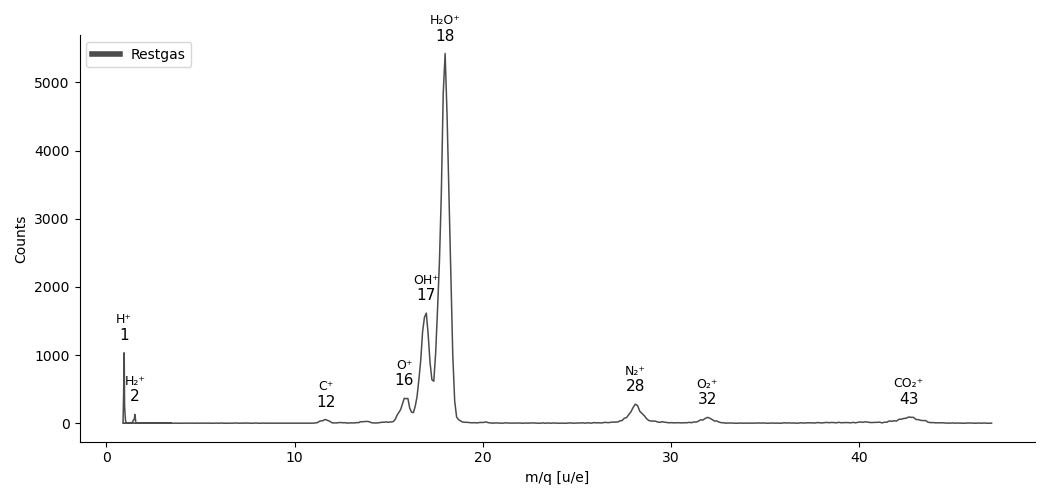
\includegraphics[width=1.05\textwidth]{Restgas.png}
    \caption[Masse-zu-Ladungsspektrum der Restgase]{Masse-zu-Ladungsspektrum der Restgase erzeugt aus dem Flugzeitspektrum in Abb. \ref{fig:rest_tof}. Die Peaks entsprechen den verschiedenen Ionen, die durch die Elektronenstoßionisation entstanden sind. Das Spektrum wurde skaliert, um die Masse zu Ladungsverhältnisse der Ionen zu bestimmen.}
    \label{fig:rest}
\end{figure}

\section{Auswertung der Positionsdaten}
Anhand der vom Detektor aufgenommenen Positionsdaten der Ionen, können Rückschlüsse auf den Entstehungsort der Ionen gezogen werden. Abbildung \ref{fig:Strahl} zeigt einen Plot dieser Daten für eine Messung mit Argonionen. Es ist zu erkennen, dass die Ionen, wie erwartet, entlang eines horizontalen Streifens entstehen, der seitlich abgeschnitten ist. Die Ionen wurden durch das 2 cm große Loch in der Deckenplatte des Beschleunigungskondesators auf den Detektor geschossen. Deshalb ist das Abbild des Elektronenstrahls seitlich begrenzt. Die Entstehungsorte der Ionen sind offensichtlich stark mit dem Strahl verbunden, was zeigt, dass die Ionen entlang des Strahls entstehen und nicht wesentlich abgelenkt werden oder aus anderen Quellen stammen.

\subsection{Annomalien}
Auffällig sind jedoch die Überhöhungen an den seitlichen Rändern des Strahls, die in Abbildung \ref{fig:Strahl3D} besonders deutlich zu erkennen sind. Außerdem ist die Länge des Abbilds von 28 mm unvorhergesehen. Bei geraden Flugbahnen der Ionen würde ein Abbild von etwa 20 mm Länge erwartet werden, entsprechend dem Loch in der Deckenplatte. Anders als bei einem Ionenstrahl, bei dem die Coloumbabstoßung eine Aufweitung bewirkt, sollte kein solcher Effekt unter der Einzelstoßbedingung auftreten. Beide dieser Effekte sollen mit der Simulation der Ionenoptik überprüft werden, um eine mögliche Erklärung zu finden. Die leichte Wölbung des Strahls war während des Experiments konstant und kann nur auf eine Ungenauigkeit der vom Detektor ermittelten Positionen zurückgeführt werden. 
\begin{figure}
    \centering
    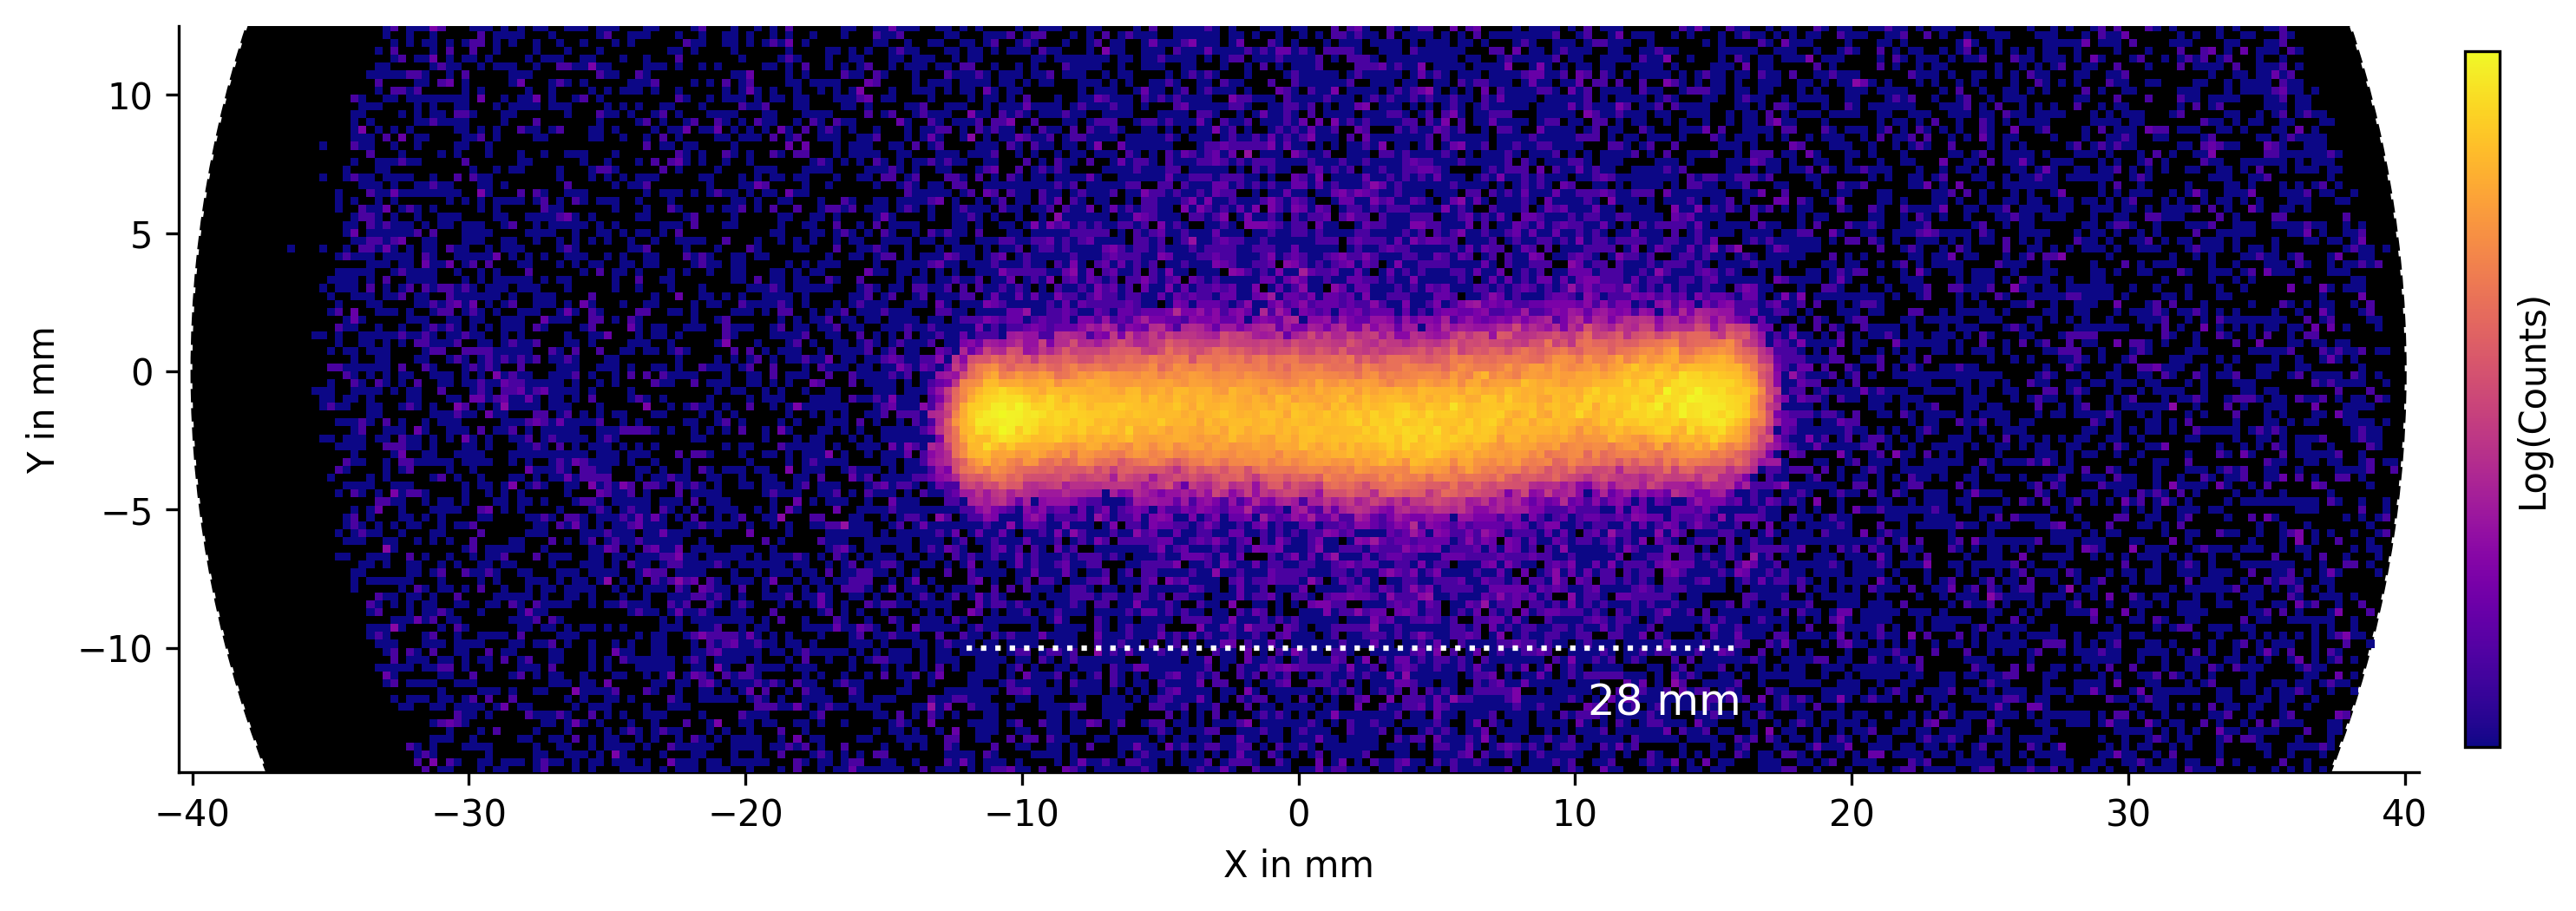
\includegraphics[width=1.05\textwidth]{Strahl.png}
    \caption[Logarithmisches Abbild des Strahls auf dem Detektor]{Positionsbestimmung der detektierten Teilche auf dem Detektor zeigt den Strahl bei einer Elektronenengie 100 eV auf dem Detektor. Die Anzahl der Treffer in einem Pixel wird logarithmisch skaliert von den Farben angegeben. Da der Detektor schief verbaut ist, wurde das Bild im Nachhinein gedreht. Das Abbild des Strahls ist seitlich begrenzt, da die Ionen durch das 2 cm große Loch in der Deckenplatte auf den Detektor gelangen. Die geometrische Größe des Detektors ist in Schwarz eingezeichnet.}
    \label{fig:Strahl} 
\end{figure}

\begin{figure}
    \centering
    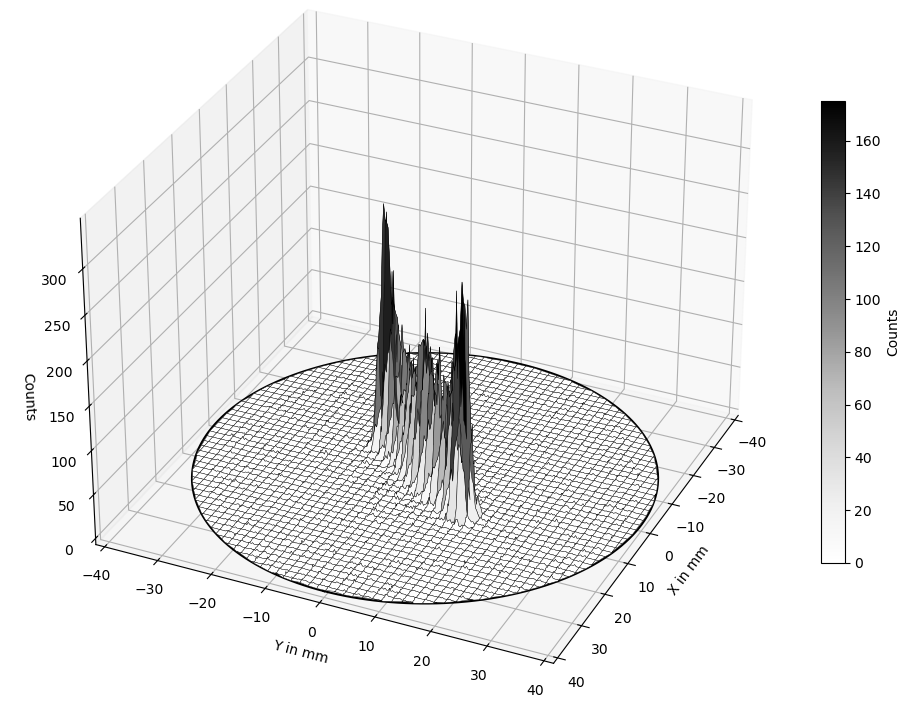
\includegraphics[width=.85\textwidth]{Strahl3D.png}
    \caption[Dreidimensionales Abbild des Strahls auf dem Detektor]{Dreidimensionales Abbild des Strahls auf dem Detektor. Die Anzahl der Treffer ist absolut dargestellt. Die Überhöhungen an den Rändern des Strahls sind gut zu erkennenbar. Das Bild zeigt die tatsächliche Ausrichtung des Detektors relativ zum Strahl.}
    \label{fig:Strahl3D} 
\end{figure}

\subsection{Ermittlung des Elektronenstrahlprofil}
Die Positionen der detektierten Ionen auf dem Detektor können genutzt werden, um das Strahlprofil, also die räumliche Verteilung der Teilchen in einem Schnitt des Strahls, zu bestimmen. Um das Strahlprofil über die ganze abgebildete Länge zu mitteln, wird Daten-Binning genutzt. Das bedeutet, dass für jede y-Koordinate in einem \textit{Bin} die Counts aller detektierten Ionen aufsummiert werden. Das Ergebnis ist ein Histogramm, das die räumliche Verteilung der Elektronen entlange der y-Achse zeigt. Das Ergebnis ist in Abb. \ref{fig:Strahlprofil} dargestellt. Für das Profil des Strahls wird eine Gauß-Verteilung erwartet, da thermische Effekte und Beugung die Position der Elektronen zufällig beeinflussen. Mit einem Fit der Daten mit einer Gauß-Funktion kann die Breite des Strahls bestimmt werden. In der Abbildung ist zu erkennen, dass die Abweichung der Daten vom Fit sehr klein ist. Über die Parameter der gefitteten Funktion kann die volle Breite bei halbem Maximum (FWHM) des Strahls bestimmt werden. Sie beträgt 2.93 mm bei 100 eV. Obwohl diese Strahlbreite in die vom Hersteller angegebene Fleckgröße von 5 mm passt, ist sie wahrscheinlich, ähnlich wie die horizontale Länge des Strahls, tatsächlich kleiner. Wenn man annimmt, dass die Vergrößerung entlang der y-Achse ähnlich der entlang der x-Achse ist, sollte der Strahl eine FWHM von etwa 2 mm aufweisen.

\begin{figure}
    \centering
    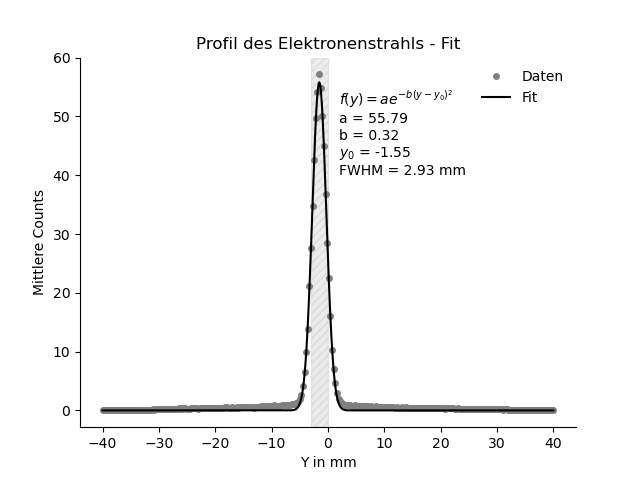
\includegraphics[width=.7\textwidth]{Strahlprofil.png}
    \caption[Gemitteltes Strahlprofil]{Gemitteltes Strahlprofil aus den Positionen der detektierten Ionen. Die Daten wurden mit einem Gaußfit gefittet, um die Breite des Strahls zu bestimmen. In grau-schraffiert eingezeichnet ist die volle Breite bei halbem Maximum (FWHM) des Strahls abgebildet.}
    \label{fig:Strahlprofil} 
\end{figure}
\cleardoublepage
\appendix
% remove header trickery
\chapter[]{Anhang}
\addcontentsline{toc}{chapter}{A\ \ Anhang}
\begin{table}[H]
    \caption{Spannungswerte bei der Konditionierung}
    \label{tab:Konditionierung}
    \begin{tabular}{lccc}
        \toprule
        Spannungsdifferenz [V] & Strom [mA] &	Widerstand [M$\Omega$] & Zeitinterval [min]\\   
        \midrule
            880  & 0,018 & 48,9 & 05:57\\
            980  & 0,021 & 46,7 & 06:39\\
            1080 & 0,024 & 45,0 & 05:36\\
            1200 & 0,028 & 42,9 & 07:26\\
            1330 & 0,032 & 41,6 & 07:20\\
            1450 & 0,036 & 40,3 & 04:13\\
            1580 & 0,040 & 39,5 & 04:41\\
            1700 & 0,044 & 38,6 & 04:43\\
            1825 & 0,048 & 38,0 & 06:01\\
            1940 & 0,052 & 37,3 & 05:10\\
            2060 & 0,056 & 36,8 & 07:45\\
            2160 & 0,059 & 36,6 & 05:57\\
            2270 & 0,063 & 36,0 & 05:59\\
            2380 & 0,068 & 35,0 & 06:16\\
            2480 & 0,071 & 34,9 & 06:27\\
            2600 & 0,071 & 36,6 & 06:02\\
            2700 & 0,080 & 33,8 & 06:46\\   
        \bottomrule     
    \end{tabular}
\end{table}
\clearpage
\section{Ergänzendes zur Simulation}
Alle Skripte, sowie die gesamte ionenoptische Simulation, die im Verlauf dieser Arbeit entwickelt wurden, stehen zur freien Verfügung und sind im GitLab der JLU Gießen unter folgendem Link zu finden: \url{https://gitlab.ub.uni-giessen.de/so9354/zerob-software}.



\begin{figure}[H]
    \centering
    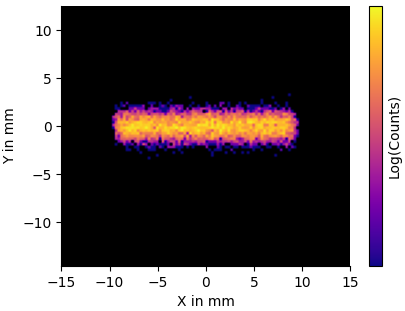
\includegraphics[width=.55\textwidth]{Pos_210.png}
    \caption[Positionsplot des konvergenten Strahls]{Positionsplot des konvergenten Strahls bei einer Flugstrecke von 210 mm.}
    \label{fig:pos_210}
\end{figure}

\begin{figure}[H]
    \centering
    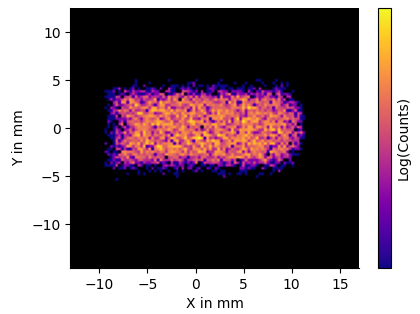
\includegraphics[width=.55\textwidth]{Pos_Forward_Bias.png}
    \caption[Positionsplot mit Vorzugsrichtung der thermischen Bewegung]{Positionsplot mit Vorzugsrichtung der thermischen Bewegung der Ionen. Die Richtungsverteilung der thermischen Bewegung (hier 1/5 eV) ist in einem Kegel um die x-Achse gegeben. Der Öffnungswinkel des Kegels beträgt 110°. Versucht wurde die Verschiebung in x-Richtung des Strahl im Expermiments nachzuvollziehen. Allerdings ist kein wesentlicher Unterschied zu Abbildung \ref{fig:sim_pos_kinetic} erkennbar.}
    \label{fig:pos_bias}
\end{figure}   


\begin{figure}[H]
    \centering
    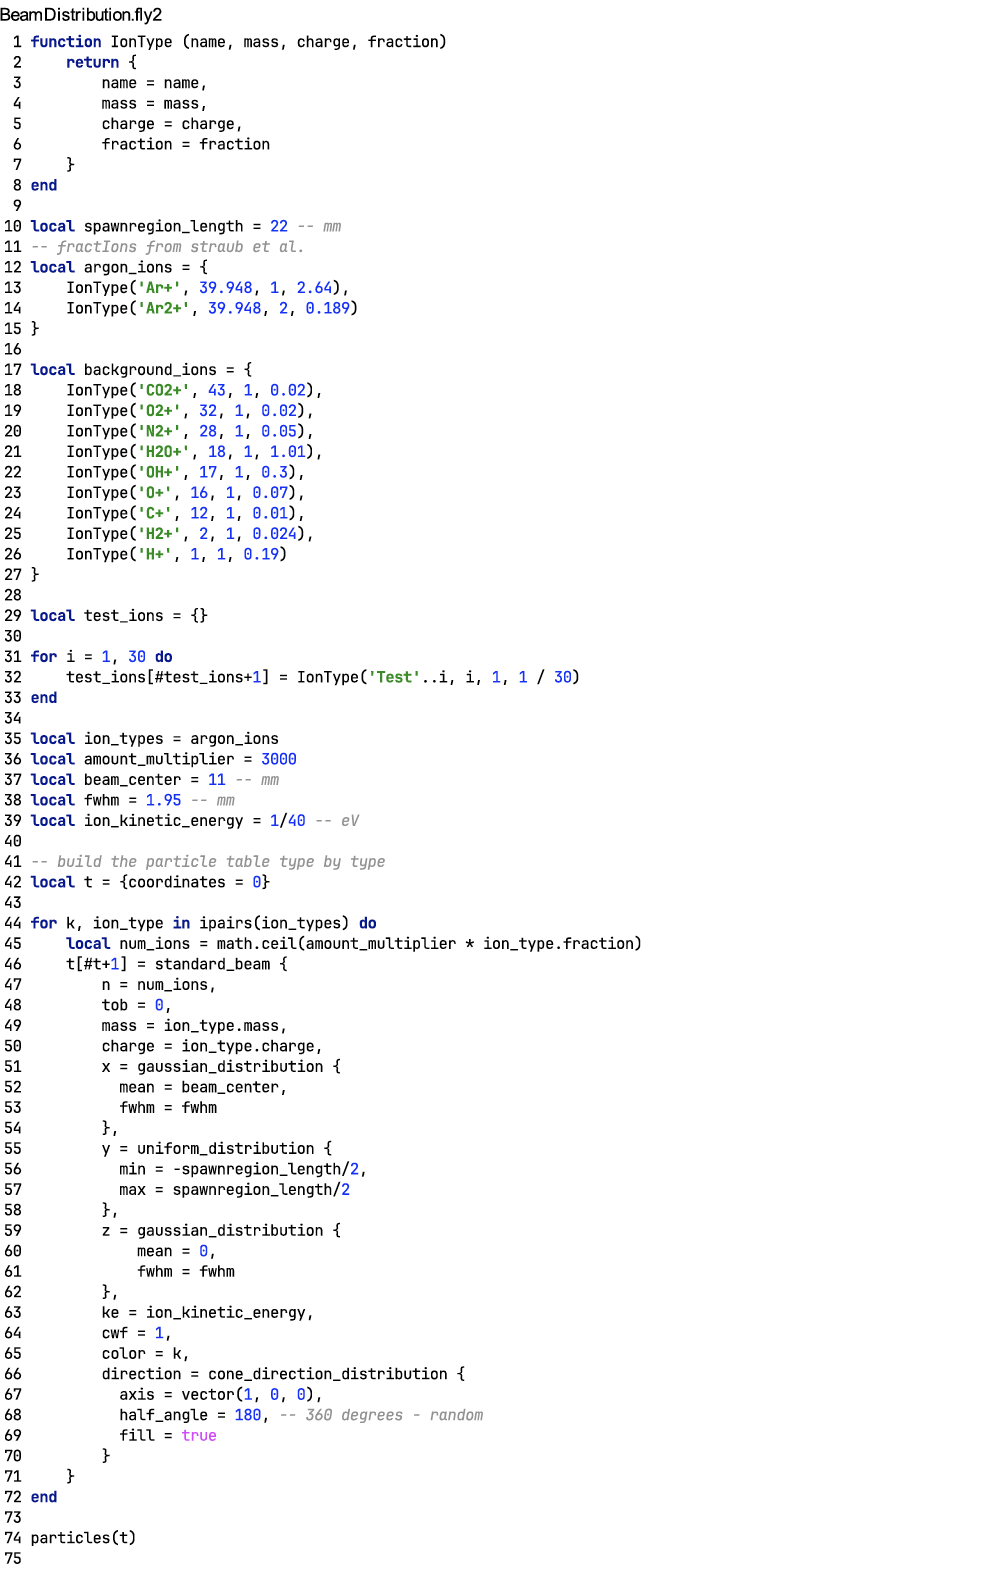
\includegraphics[width=1.05\textwidth]{Fly2.png}
    \caption[Ionenverteilung .fly2-File]{.fly2-File zur Definition der Ionenverteilung in \textit{SIMION} in der Programmiersprache Lua.}
    \label{fly2}
\end{figure}


\fontsize{12pt}{12pt}\selectfont

% Change Bibliography to References
\renewcommand\bibname{Literaturverzeichnis}
\clearpage
\phantomsection
\addcontentsline{toc}{chapter}{Literaturverzeichnis}

\printbibliography


\end{document}